%import template
\documentclass[a4paper, landscape , 8pt]{scrartcl}

% use language german
\usepackage[T1]{fontenc}
\usepackage[utf8]{inputenc}
\usepackage[english, ngerman]{babel} % \selectlanguage{english} if  needed
\usepackage{lmodern} % use modern latin fonts

% format
\usepackage{geometry}
\geometry{top=2cm,left=1.4cm,right=1.4cm}
\textheight = 520pt

%autor
\usepackage{authblk}

%tabular
\usepackage{tabularx}

% math
\usepackage{amsmath}
\usepackage{amssymb}
\usepackage{amsfonts}
\usepackage{enumitem}

% graphic
\usepackage{graphicx}
\graphicspath{{graphic/}} 

%colors
% \usepackage{xcolor}

% Multi Columns
\usepackage{multicol}

%compact items
\setlist{topsep=0pt, leftmargin=3mm, nolistsep}
\setlength{\parindent}{0cm}

%define header and footer
\usepackage{fancyhdr}
\pagestyle{fancy}

\fancyhead[RO]{\AUTHOR| \INSTITUTE}
\fancyhead[LO]{\TITLE}
\fancyfoot[RO]{\today}
\fancyfoot[LO]{Created with \LaTeX}
\renewcommand\headrulewidth{0pt}
\renewcommand\footrulewidth{0pt}
\headsep = -2pt
\footskip = 0pt


% Define Section Format
\usepackage{sectsty}
\usepackage{titlesec}
\usepackage[dvipsnames]{xcolor}

\titleformat{name=\section}[block]{\sffamily\normalsize}{}{0pt}{\colorsection}
\titlespacing*{\section}{0pt}{0pt}{0pt}
\newcommand{\colorsection}[1]{%
	\colorbox{sectioncolor!80}{\parbox{0.98\linewidth}{\vspace{-1pt}\color{white}\ #1 \vspace{-2pt}}}}

% Define Subsection Format
\titleformat{name=\subsection}[block]{\sffamily\small}{}{0pt}{\colorsubsection}
\titlespacing*{\subsection}{0pt}{0pt}{0pt}
\newcommand{\colorsubsection}[1]{%
	\colorbox{subsectioncolor!80}{\parbox{0.98\linewidth}{\vspace{-1pt}\color{black}\ #1 \vspace{-2pt}}}}

% Define SubSubsection Format
\titleformat{name=\subsubsection}[block]{\sffamily\small}{}{0pt}{\colorsubsubsection}
\titlespacing*{\subsubsection}{0pt}{0pt}{0pt}
\newcommand{\colorsubsubsection}[1]{%
	\colorbox{subsubsectioncolor!60}{\parbox{0.98\linewidth}{\vspace{-1pt}\color{black}\ #1 \vspace{-2pt}}}}


%define color
\definecolor{sectioncolor}{HTML}{052639}
\definecolor{subsectioncolor}{HTML}{468189}
\definecolor{subsubsectioncolor}{HTML}{8DB9B1}
\definecolor{b}{RGB}{0, 115, 192 } %Default highlite color
\definecolor{p}{RGB}{0, 43, 54} %Dark page color
\definecolor{t}{RGB}{131, 148, 150} %Dark text color
\definecolor{darkgreen}{RGB}{0,150,0}
\definecolor{dkgreen}{rgb}{0,0.6,0}
\definecolor{gray}{rgb}{0.5,0.5,0.5}
\definecolor{mauve}{rgb}{0.58,0,0.82}
\definecolor{DarkPurple}{rgb}{0.4, 0.1, 0.4}
\definecolor{DarkCyan}{rgb}{0.0, 0.5, 0.4}
\definecolor{LightLime}{rgb}{0.3, 0.5, 0.4}
\definecolor{Blue}{rgb}{0.0, 0.0, 1.0}
\definecolor{h}{RGB}{1, 101, 163}

% Code Listings
\usepackage{listings}
\usepackage{color}
\usepackage{beramono}
\usepackage{hyperref}
\hypersetup{
    colorlinks,
    linkcolor={black},
    citecolor={blue!50!black},
    urlcolor={blue!80!black}
}

\definecolor{bluekeywords}{rgb}{0,0,1}
\definecolor{greencomments}{rgb}{0,0.5,0}
\definecolor{redstrings}{rgb}{0.64,0.08,0.08}
\definecolor{xmlcomments}{rgb}{0.5,0.5,0.5}
\definecolor{types}{rgb}{0.17,0.57,0.68}
\definecolor{codeBackground}{RGB}{250,250,250}


\lstdefinestyle{JS}{
language=java,
backgroundcolor = \color{codeBackground},   % color for the background.
basicstyle=\ttfamily\scriptsize,            % font size/family/etc. for source
keywordstyle=\color{RoyalBlue}\ttfamily,    % style of keywords in source language
stringstyle=\color{darkgreen}\ttfamily,     % style of strings in source language
commentstyle=\color{DarkPurple!60}\ttfamily,% style of comments in source language
escapeinside={£}{£},                        % specify characters to escape from source code to LATEX
showspaces=false,                           % emphasize spaces in code (true/false)
showstringspaces=false,
showtabs=false,                             % emphasize tabulators in code (true/false)
numbers=none,                               % position of line numbers (left/right/none)
numberstyle=\tiny\color{darkgray}\ttfamily, % style used for line-numbers
stepnumber=1,                               % distance of line-numbers from the code
tabsize=1,                                  % default tabsize
breaklines=true,                            % automatic line-breaking
breakatwhitespace=true,                     % sets if automatic breaks should only happen at whitespaces
frame=single,                               % showing frame outside code (none/leftline/topline/bottomline/lines/single/shadowbox)
xleftmargin=3pt,
xrightmargin=1pt,
frameround=tttt,                            % enable round corners
rulecolor = \color{lightgray},              % Specify the colour of the frame-box
aboveskip = 1pt,
belowskip = 1pt,
captionpos = b                              % position of caption (t/b)
}
\lstset{
	style=JS
	% literate=  % Allow for German characters in lstlistings.
	% {Ö}{{\"O}}1
	% {Ä}{{\"A}}1
	% {Ü}{{\"U}}1
	% {ü}{{\"u}}1
	% {ä}{{\"a}}1
	% {ö}{{\"o}}1}
}




% Theorems \begin{mytheo}{title}{label}
\usepackage{tcolorbox}
\tcbuselibrary{theorems}
\newtcbtheorem[number within=section]{definiton}{Definition}%
{fonttitle=\bfseries}{def}
\newtcbtheorem[number within=section]{remember}{Merke}%
{fonttitle=\bfseries}{rem}
\newtcbtheorem[number within=section]{hint}{Hinweis}%
{fonttitle=\bfseries}{hnt}

% new section -> new page
% \let\stdsection\section
% \renewcommand\section{\clearpage\stdsection}

% Front page
\newcommand{\AUTHOR}{Marius Zindel }
\newcommand{\INSTITUTE}{Hochschule für Technik Rapperswil}

%dotted rule
\usepackage{dashrule}
\usepackage{tikz}
\usetikzlibrary{decorations.markings}
\newcommand{\drule}[3][0]{
	\tikz[baseline]{\path[decoration={markings,
	mark=between positions 0 and 1 step 2*#3
	with {\node[fill, circle, minimum width=#3, inner sep=0pt, anchor=south west] {};}},postaction={decorate}]  (0,#1) -- ++(#2,0);}}


%no indentation
\setlength{\parindent}{0cm}

\usepackage{lipsum}

% DocInfo
\newcommand{\SUBJECT}{}
\newcommand{\TITLE}{Cheat Sheet Informations und Codierungs Theorie}

\begin{document}

%import front page
% \input{./front.tex}

%do multicols
\begin{multicols*}{5}
    \setlength{\columnseprule}{0.4pt}
		\footnotesize
		
%import tableofcontents
% 
%Table of contents
\tableofcontents

% don't show \subsubsection in \tableofcontents
\setcounter{tocdepth}{2}

	%! Author = mariuszindel
%! Date = 25.01.21

\section{Signalparameter}


\subsection{Was ist Information?}
\begin{center}
    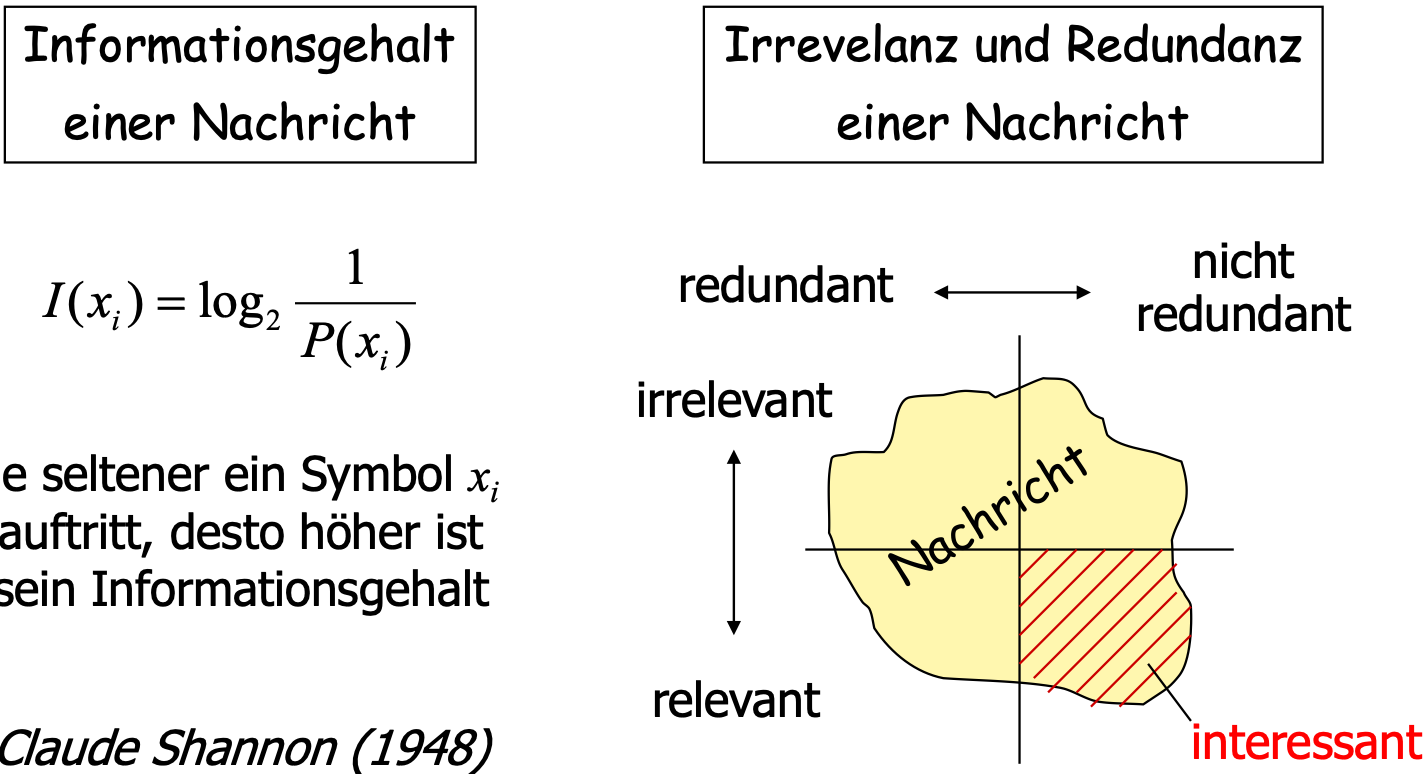
\includegraphics[width=\linewidth]{graphic/signalparameter/wasist.png}
\end{center}
\vspace{-8pt}


\subsection{Non-Return-to-Zero Code (NRZ)}
\subsubsection{gleichstrombehaftet, keine Taktinformation}
\begin{center}
    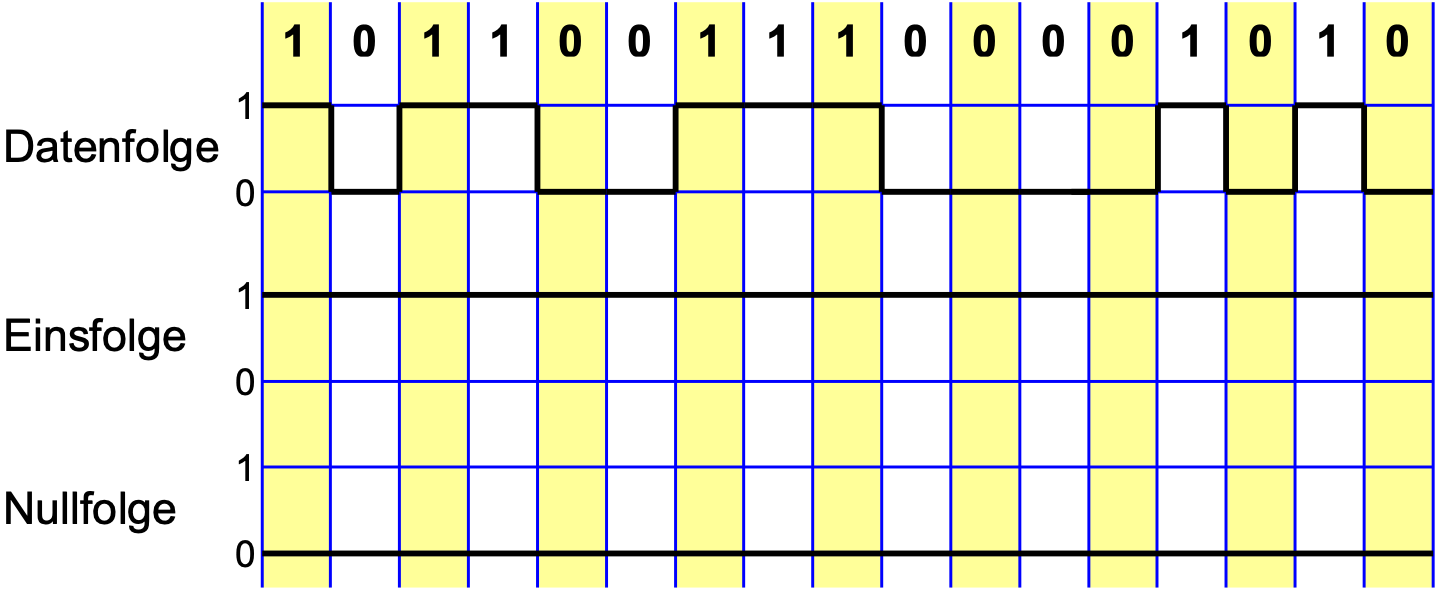
\includegraphics[width=\linewidth]{graphic/signalparameter/gleichstrombehaftet.png}
\end{center}
\vspace{-8pt}

\subsubsection{gleichstromfrei, volle Taktinformation}
\begin{center}
    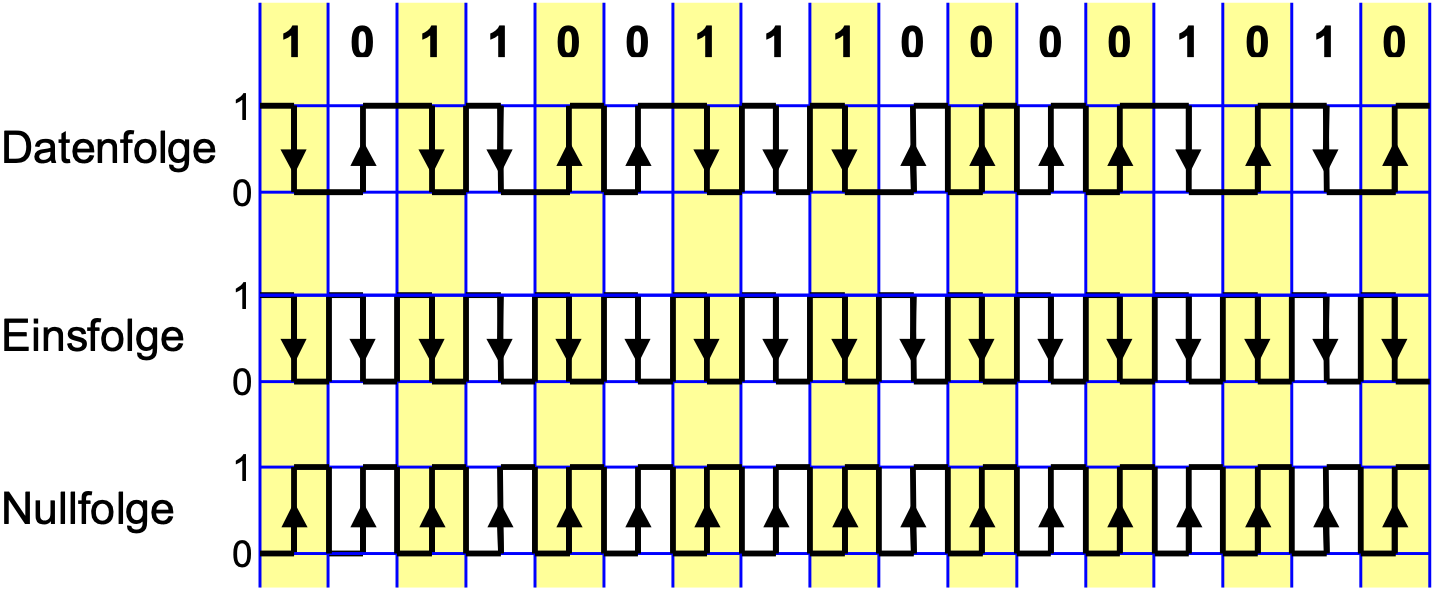
\includegraphics[width=\linewidth]{graphic/signalparameter/gleichstromfrei.png}
\end{center}
\vspace{-8pt}

\subsection{Pegelberechnung}
 \begin{center}
     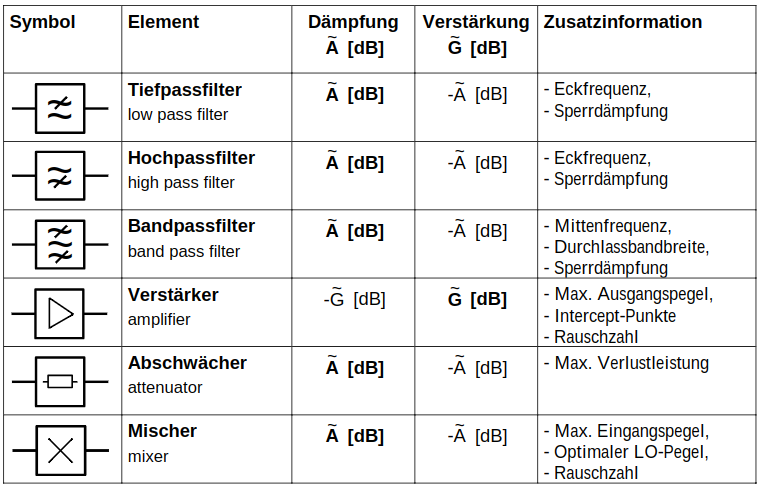
\includegraphics[width=\linewidth]{graphic/signalparameter/pegelplan.png}
 \end{center}
 \vspace{-8pt}

\subsubsection{Maximaler Ausgangspegel (z.B für Vorverstärker)}
$P=\frac{\hat{U}^{2}}{2 R}=\frac{(1 \mathrm{~V})^{2}}{2 \cdot 50 \Omega}=10 \mathrm{~mW} $\\
$\quad \widetilde{P}[\mathrm{dBm}]=10 \cdot \log \frac{P}{1 \mathrm{~mW}}=\underline{\underline{10 \mathrm{dBm}}}$


\subsubsection{Signaldynamik}
Differenz zwischen höchst- und tiefstmöglichen Pegel
\vspace{-8pt}
\begin{center}
    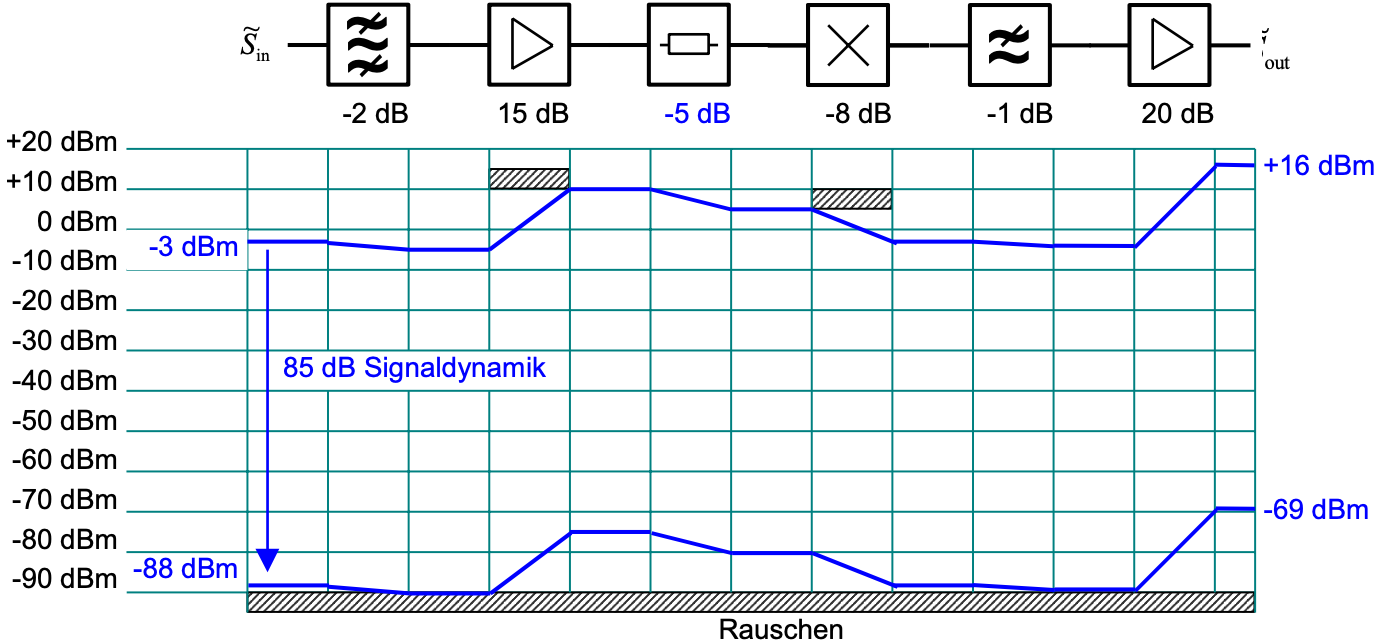
\includegraphics[width=\linewidth]{graphic/signalparameter/uebung.png}
\end{center}
\vspace{-8pt}


\subsubsection{Spannungseffektivwert}
$\widetilde{P}_{\max }=+16 \mathrm{dBm} \rightarrow \quad P_{\max }=40 \mathrm{~mW} $\\
$\quad U_{\max }=\sqrt{R P_{\max }}=\sqrt{50 \Omega \cdot 0.04 \mathrm{~W}}=1.41 \mathrm{~V}_{\mathrm{eff}}$


\subsection{Watt $\rightarrow$ dBm}
$L_{P}[\mathrm{dBm}]=10 \log _{10}\left(\frac{P}{1 \mathrm{~mW}}\right)$
\vspace{-8pt}
\begin{center}
    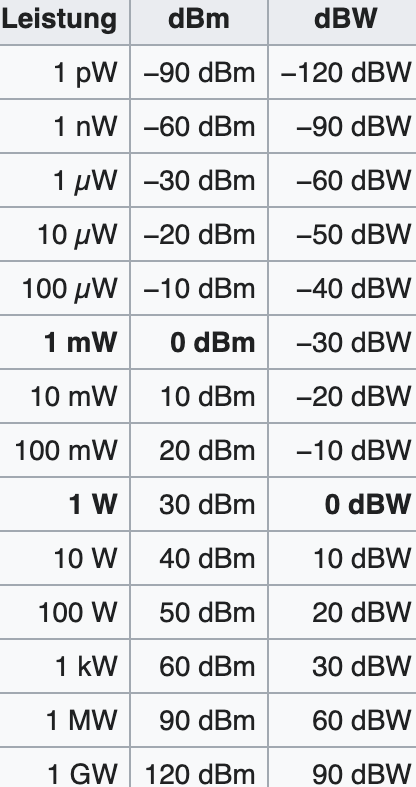
\includegraphics[scale=.3]{graphic/signalparameter/dbm-tabelle.png}
\end{center}
\vspace{-8pt}


\subsection{dBm $\rightarrow$ Watt}
$P[\mathrm{~mW}]=10^{\left(\frac{L_{P}[\mathrm{dBm}]}{10}\right)} \cdot 1 \mathrm{~mW}$

	%! Author = mariuszindel
%! Date = 25.01.21

\section{Signale}


\subsection{Periodendauer}
Die Periodendauer hat den Formelbuchstaben T und die Einheit Sekunde s.\\
$T[s] = \frac{1}{f}$

\subsection{Frequenz}
Die Frequenz hat den Formelbuchstaben f und die Einheit Hertz Hz.\\
$f[Hz] = \frac{1}{T}$



\subsection{Dauer und Bandbreite von Einzelpulsen}
\subsubsection{Vorgehen Amplitudendichte}
\textbf{Fragestellung:} Wie kann S(0), d.h. die Amplitudendichte bei der Frequenz f=0 Hz, einfach aus dem Verlauf des Pulses berechnet werden? Geben Sie die Formel für S(0), sowie den numerischen Wert in [V/Hz] an.\\
\\
\textbf{Lösung:} $S(0)=\int_{-\infty }^{\infty}s(t)dt=\int_{-T}^{T}s(t)dt=AT$ \\
\\
d.h. die Gesamtfläche unter der Dreiecksfunktion s(t).\\
\\
\textbf{Hinweis:} \\
Bei Recktecksignalen wäre es $2*AT$\\
Bei ms führt es zu mV/Hz

\subsubsection{Energie berechnen}
$E=\int_{-\infty}^{\infty}\frac{s^2(t)}{R}dt=\frac{1}{R}\int_{-\infty}^{\infty}s^2(t)dt=\frac{3}{4}*\frac{A^2T}{R}$
\\
\\
Achtung: 3/4 und T ist modular \\
\\
\textbf{Hinweis:} Resultat wenn ms dann mWs (Beispiel: 3/4mWs = 0.75mJ)

\subsubsection{Dauer eines Pulses berechnen}
\textbf{Formel:} $E=\frac{A^2\tau}{R}=\frac{3}{4}*\frac{A^2T}{R}$ \\
\textbf{nach $\tau$ auflösen $\tau$ in ms oder s}\\
\\
Achtung: 3/4 und T ist modular

\subsubsection{Bandbreite}
\textbf{Formel:} $E=\frac{|S(0)|^2*B}{R}=\frac{A^2T^2B}{R}=\frac{3}{4}*\frac{A^2T}{R}$\\ $B=\frac{3}{4}*\frac{1}{T}$ und damit $B=\frac{3}{4}kHz=0.75kHz$\\
\\
Achtung: 3/4 und T ist modular

\subsubsection{Zeit-Bandbreitenprodukt}
Wie gross ist das Zeit-Bandbreitenprodukt B\tau ?\\
\\
\textbf{Formel:} $B\tau=\frac{3}{4}*\frac{1}{T}*\frac{3}{4}*T$
\\
\\
Achtung: 3/4 und T ist modular
\\
\textbf{Hinweis:} kHz und ms lösen sich auf = keine Masseinheit


% \subsection{Frequenzspektrum}


% \subsection{Analyse der Spektrallinien}


% \subsection{Signalleistung im Frequenz- und Zeitbereich}


% \subsection{Logarithmische Spektrumsdarstellung}


% \subsection{Zeitverschobene periodische Signale}
	%! Author = mariuszindel
%! Date = 25.01.21

\section{Leitungscodierung}

\subsection{Übersicht}
\subsubsection{Nur Nullstellen}
    \begin{tabular}{|l|l|l|l|l|}
        \hline
        \multirow{2}{*}{Leitungscode} & \multicolumn{2}{l|}{DC-Freiheit} & \multicolumn{2}{l|}{Taktinf} \\ \cline{2-5}
        & Ja             & Nein            & Ja               & Nein              \\ \hline
        Bipolarer NRZ            &                & X               &                  & X                 \\ \hline
        Unipolarer NRZ           & X               &                &                 &  X                 \\ \hline
        Unipolarer NRZ Mark      & *              &  *               &                 &  X                 \\ \hline
        Bipolarer Manchester     & X              &                 & X                &                   \\ \hline
        Unipolarer Manchester    &               &  X               & X                &                   \\ \hline
        Bipolarer AMI            & X              &                 &                 &  X                 \\ \hline
        Unipolarer RZ			 &	X			  & 			   & 				&	X				\\ \hline
    \end{tabular}
*Nicht entscheidbar kommt auf vorheriges Zeichen an

\subsubsection{Nur Einsstellen}
    \begin{tabular}{|l|l|l|l|l|}
        \hline
        \multirow{2}{*}{Leitungscode} & \multicolumn{2}{l|}{DC-Freiheit} & \multicolumn{2}{l|}{Taktinf} \\ \cline{2-5}
        & Ja             & Nein            & Ja               & Nein              \\ \hline
        Bipolarer NRZ            &                & X               &                  & X                 \\ \hline
        Unipolarer NRZ           &                & X               &                  & X                 \\ \hline
        Unipolarer NRZ Mark      & X              &                 & X                &                   \\ \hline
        Bipolarer Manchester     & X              &                 & X                &                   \\ \hline
        Unipolarer Manchester    & X              &                 & X                &                   \\ \hline
        Bipolarer AMI            & X              &                 & X                &                   \\ \hline
        Unipolarer RZ			 &				  & X		       & X				&					\\ \hline
    \end{tabular}

\subsubsection{Unipolarer Non-Return-to-Zero Code (NRZ)}
\begin{center}
    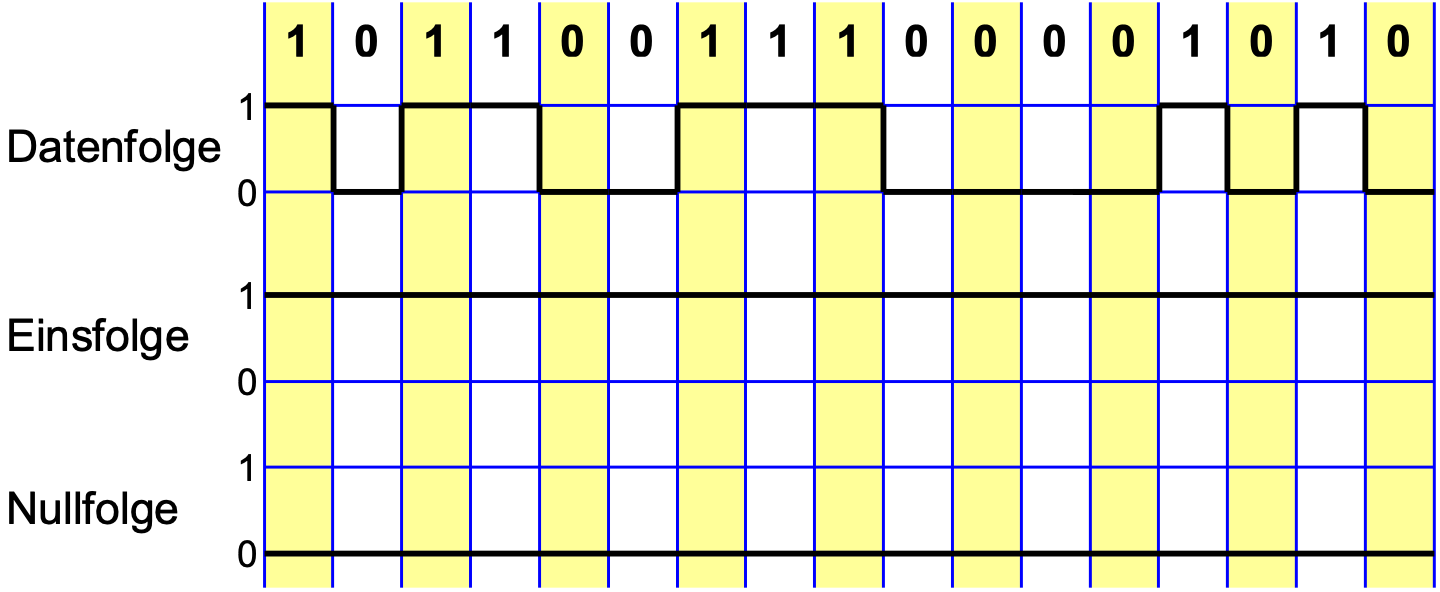
\includegraphics[width=\linewidth]{graphic/signale_analyisieren/Unipolarer Non-Return-to-Zero Code (NRZ).png}
\end{center}
\vspace{-8pt}
\begin{itemize}
    \item Gleichspannungsanteil, auch bei Random-Daten
    \item Verlust des Taktes bei langen Eins- und Nullfolgen
    \item Datenfolge enthält nicht direkt Frequenzanteile bei der Taktfrequenz
\end{itemize}


\subsubsection{Bipolarer Non-Return-to-Zero Code (NRZ)}
\begin{center}
    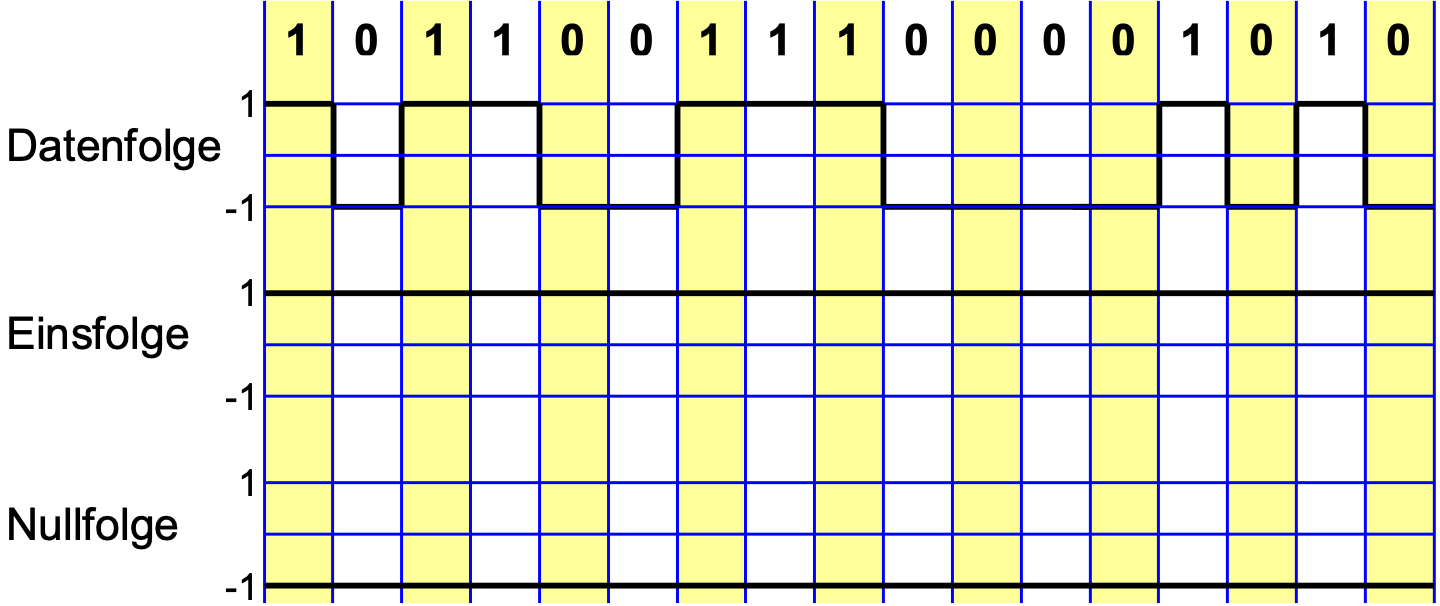
\includegraphics[width=\linewidth]{graphic/signale_analyisieren/Bipolarer Non-Return-to-Zero Code (NRZ).png}
\end{center}
\vspace{-8pt}
\begin{itemize}
    \item Kein Gleichspannungsanteil bei Random-Daten
    \item Gleichspannungsanteil bei langen Eins- und Nullfolgen
    \item Verlust des Taktes bei langen Eins- und Nullfolgen
\end{itemize}


\subsubsection{NRZ Mark Code  (Differentielle Codierung)}
\begin{center}
    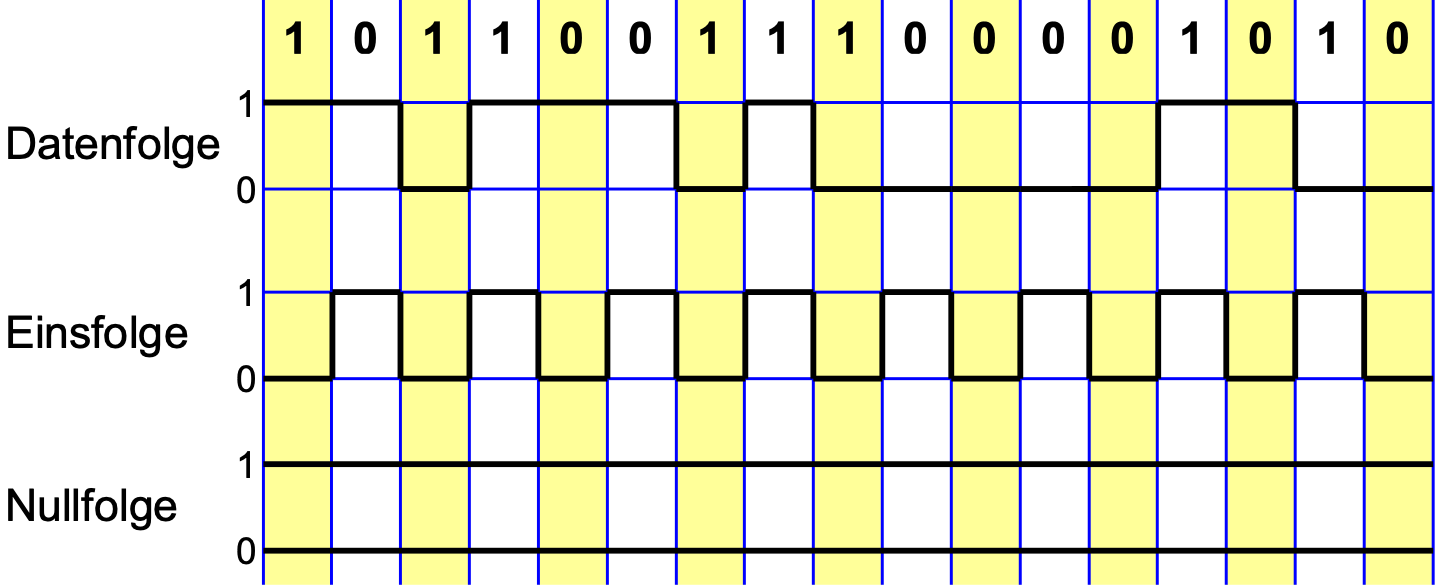
\includegraphics[width=\linewidth]{graphic/signale_analyisieren/NRZ Mark Code Differentielle Codierung.png}
\end{center}
\vspace{-8pt}
\begin{itemize}
    \item Robust gegen Vertauschen der Polarität (a/b Klemmen, absolute Phasenlage)
    \item Verlust des Taktes bei langen Nullfolgen
\end{itemize}


\subsubsection{Return-to-Zero Code (RZ)}
\begin{center}
    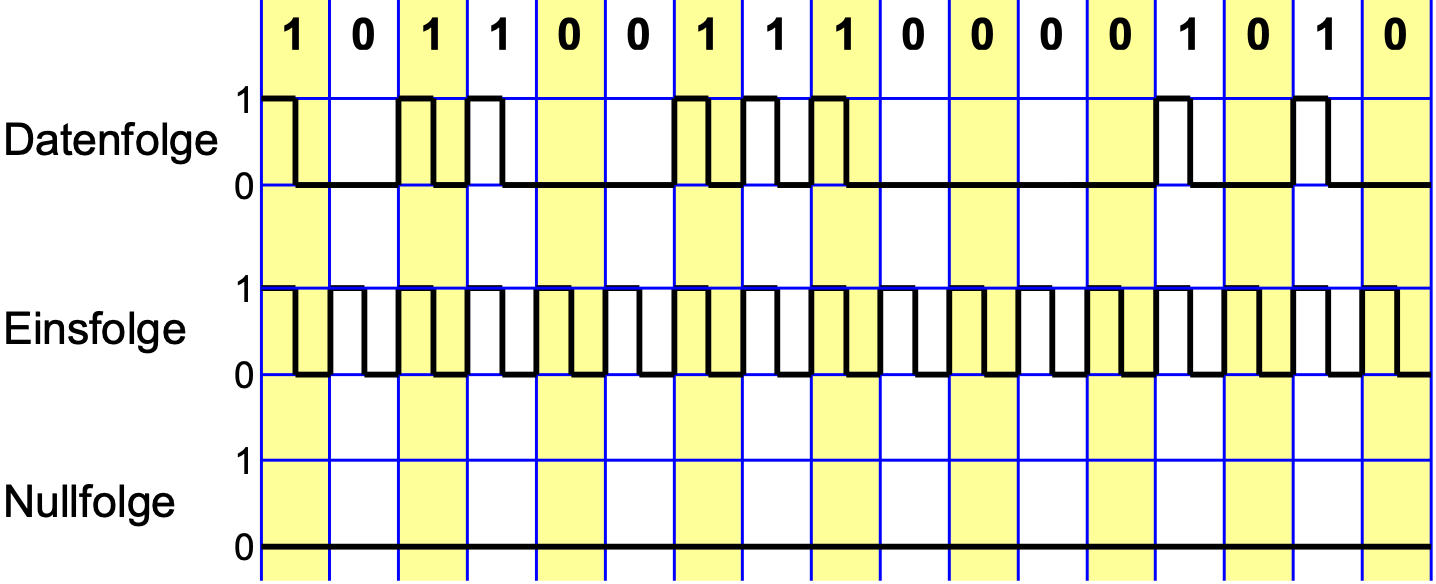
\includegraphics[width=\linewidth]{graphic/signale_analyisieren/Return-to-Zero Code (RZ).png}
\end{center}
\vspace{-8pt}
\begin{itemize}
    \item Datensignal enthält direkt Frequenzanteile bei der Taktfrequenz
    \item Durch Halbierung der Bitdauer Verdoppelung des Bandbreitenbedarfs
    \item Verlust des Taktes bei langen Nullfolgen
\end{itemize}


\subsubsection{Bi-Phase oder Manchester Code (Ethernet)}
\begin{center}
    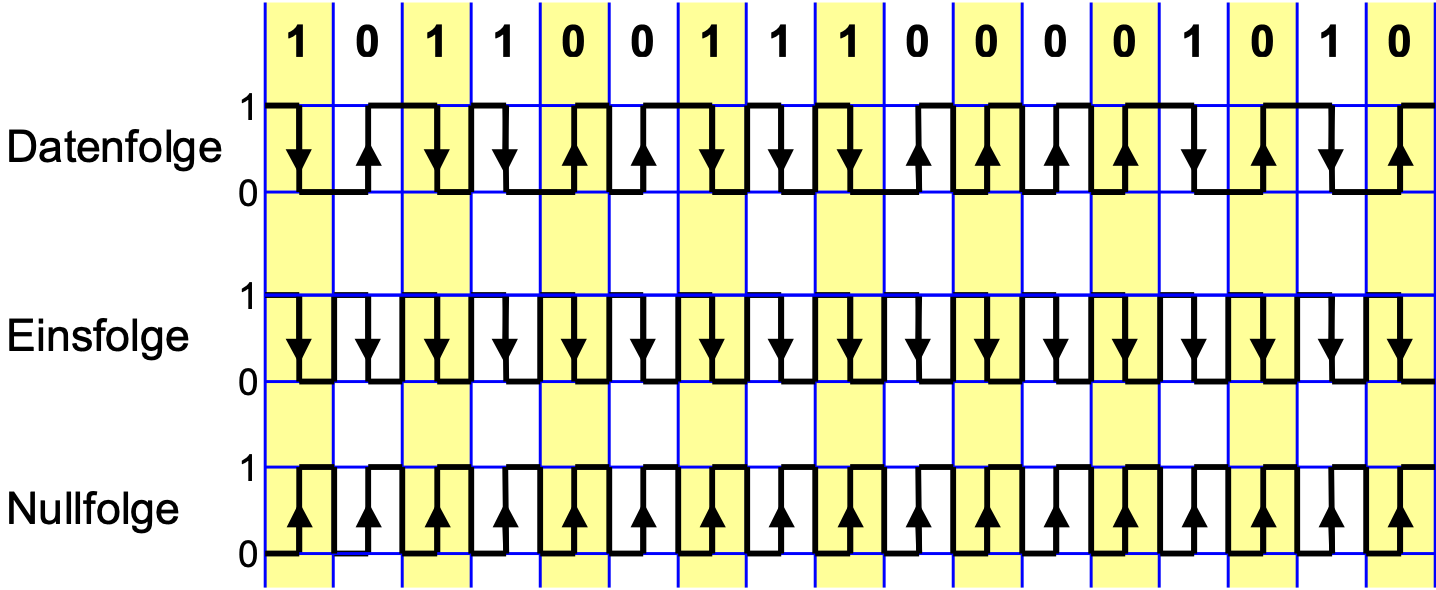
\includegraphics[width=\linewidth]{graphic/signale_analyisieren/Bi-Phase oder Manchester Code.png}
\end{center}
\vspace{-8pt}
\begin{itemize}
    \item Takt ist in jedem Datenbit vorhanden
    \item Bei bipolarem Code ist jedes Datenbit gleichspannungsfrei
    \item Durch Halbierung der Bitdauer Verdoppelung des Bandbreitenbedarfs
\end{itemize}

\subsubsection{Alternate Mark Inversion Code (AMI)}
\begin{center}
    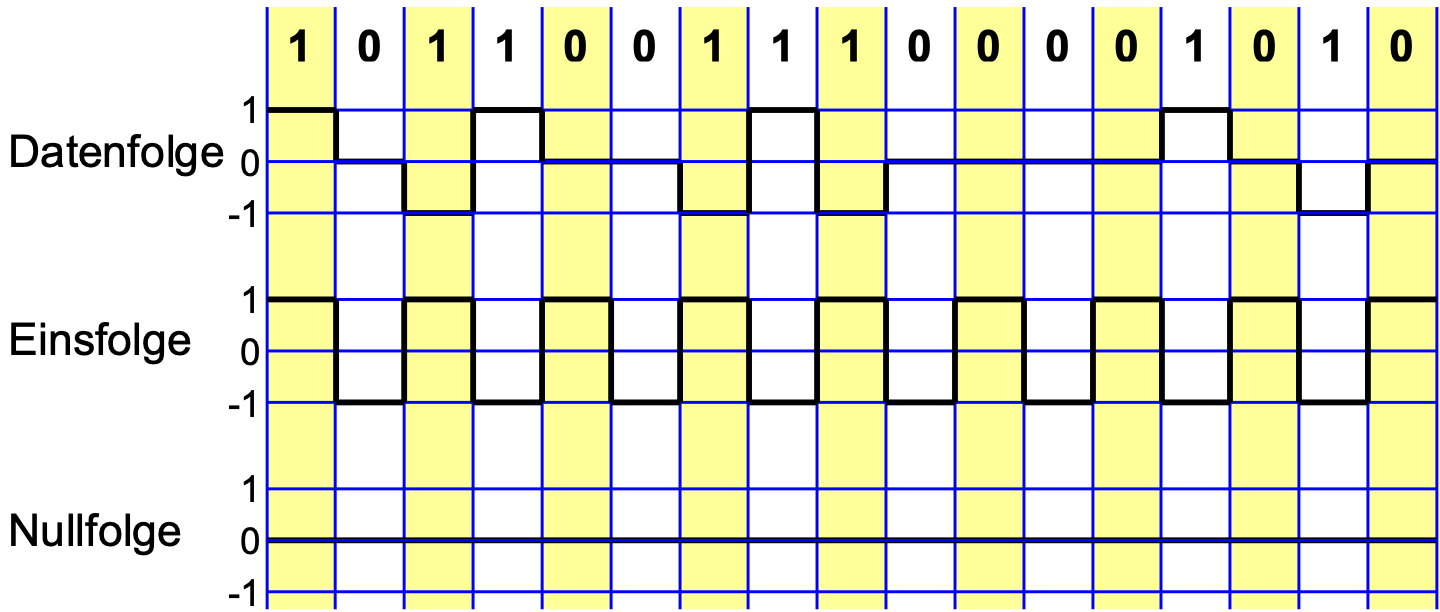
\includegraphics[width=\linewidth]{graphic/signale_analyisieren/Alternate Mark Inversion Code (AMI).png}
\end{center}
\vspace{-8pt}
\begin{itemize}
    \item Ternärer Code mit drei Spannungspegel
    \item Dank Alternierung Gleichspannungsfreiheit
    \item Verlust des Taktes bei langen Nullfolgen
\end{itemize}


\subsubsection{Scrambling}
\begin{center}
    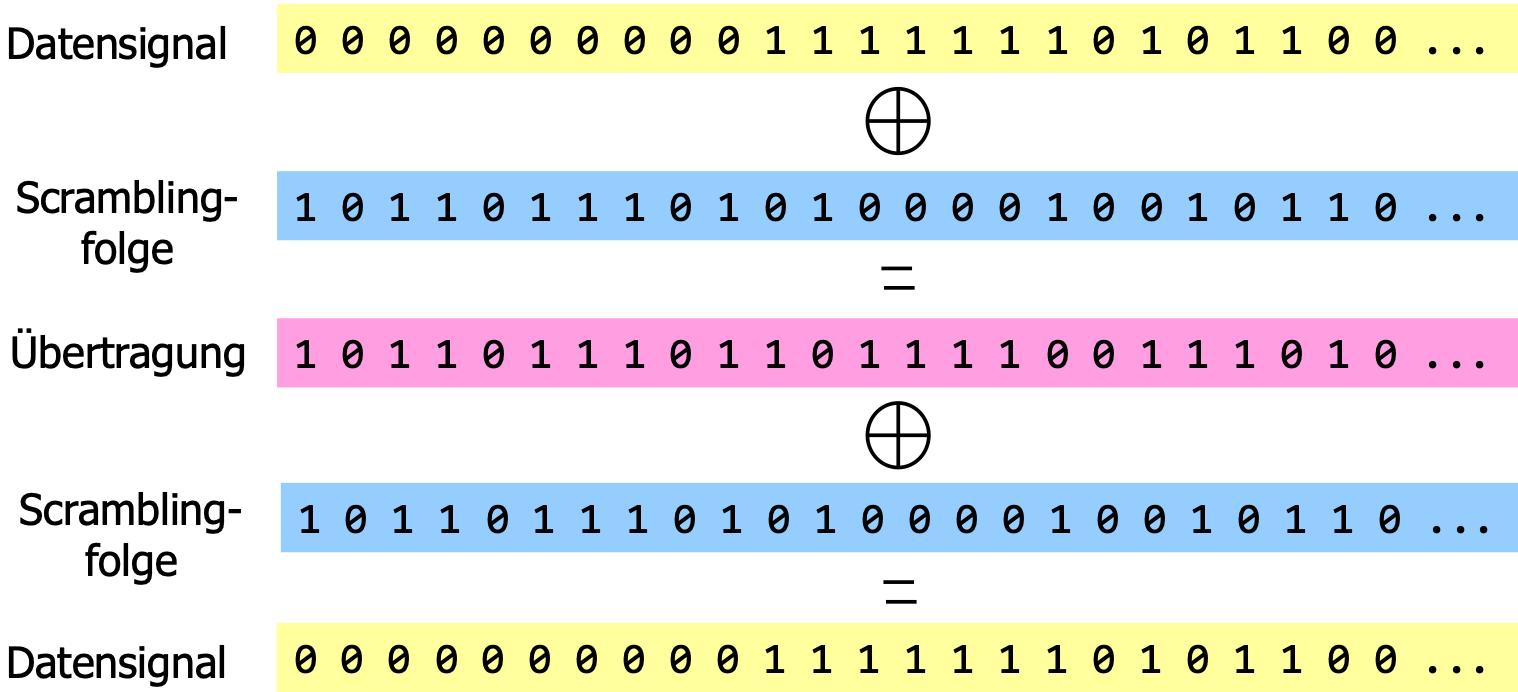
\includegraphics[width=\linewidth]{graphic/signale_analyisieren/Scrambling.png}
\end{center}
\vspace{-8pt}
\begin{itemize}
    \item Pseudozufällige Scramblingfolge z.B. aus rückgekoppeltem Schieberegister
    \item Eliminierte lange Null- und Einsfolgen
    \item Scrambler-Synchronisation setzt meist Rahmenstruktur der Daten voraus
\end{itemize}



%\section{Zweiseitiges Spektrum}
%TODO
	%! Author = mariuszindel
%! Date = 25.01.21

\section{Signale und Rauschen}
	%! Author = mariuszindel
%! Date = 25.01.21

\section{Modulationen}

\subsection{Amplitudenmodulation}
\begin{center}
    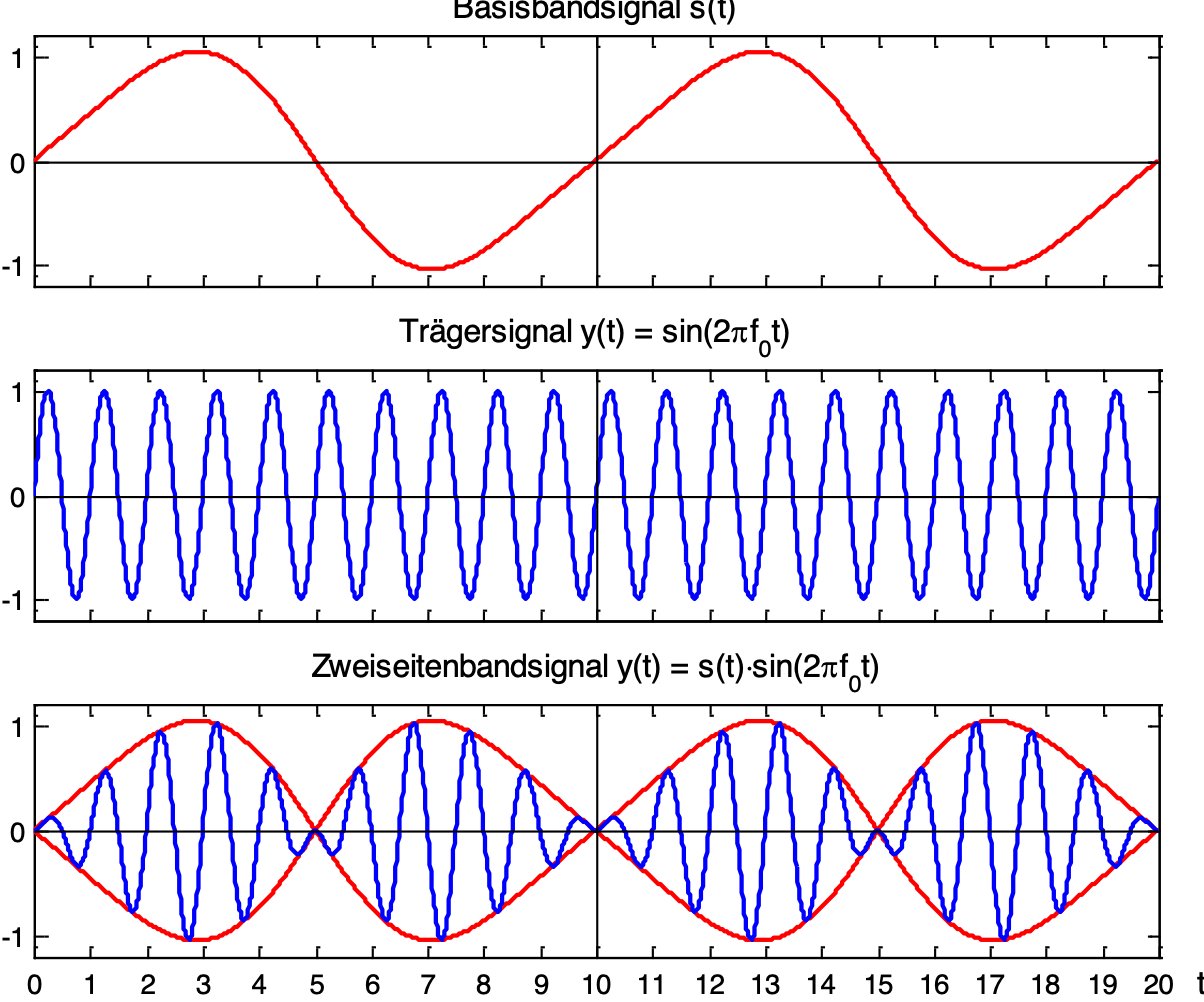
\includegraphics[width=\linewidth]{graphic/fourier/Amplitudenmodulation.png}
\end{center}
\vspace{-8pt}

\subsubsection{Oberes und Unteres Seitenband}
\begin{center}
    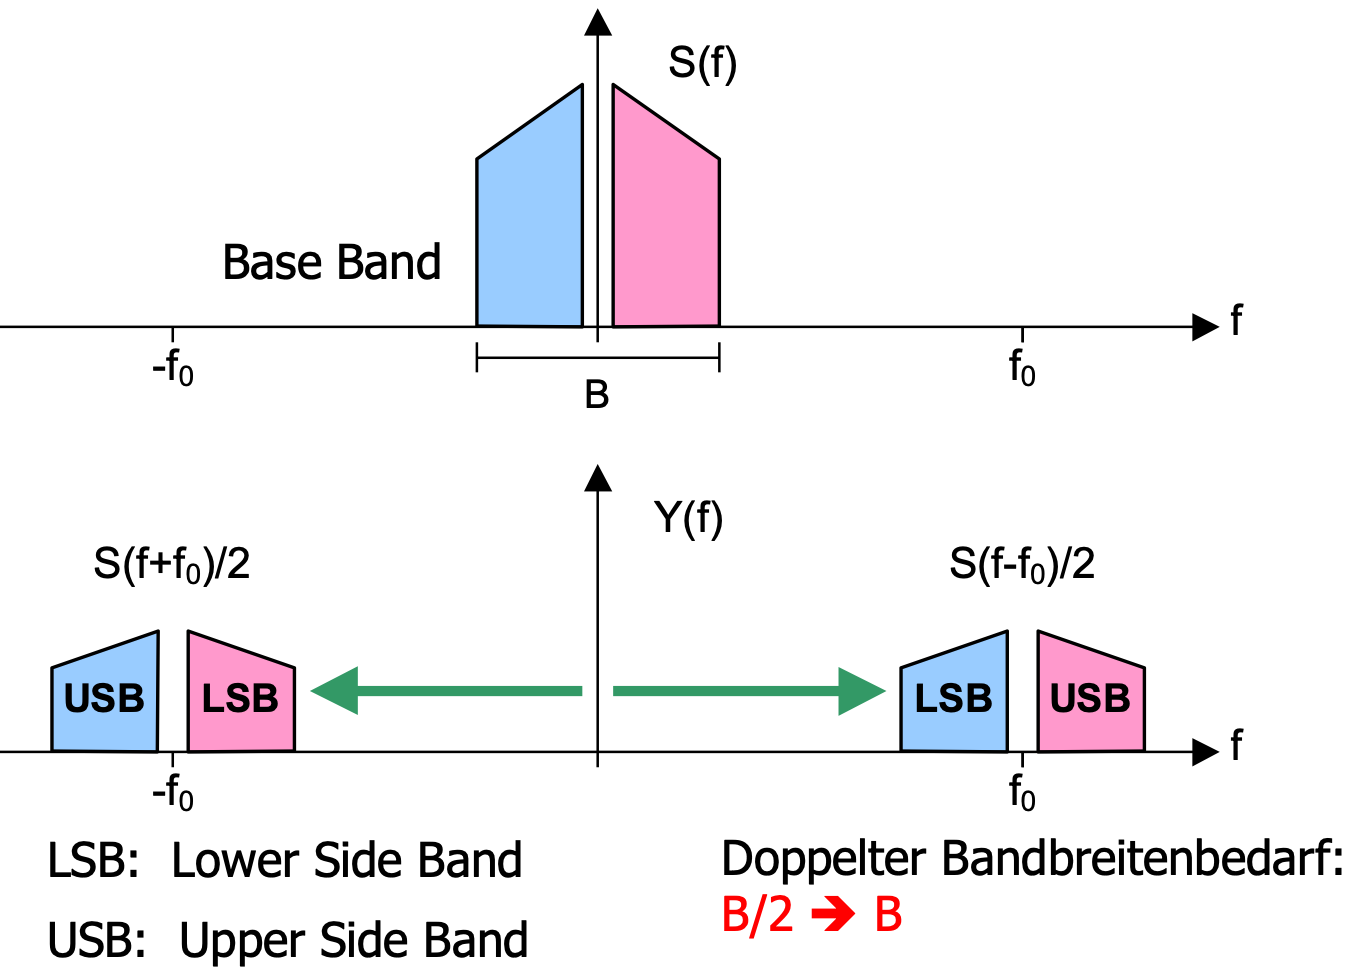
\includegraphics[width=\linewidth]{graphic/fourier/Oberes und Unteres Seitenband.png}
\end{center}
\vspace{-8pt}

\subsection{Tonhöhenverschiebung}
\subsubsection{Lösung 1:}
\begin{itemize}
    \item Elimination des oberen Seitenbandes (USB) durch ein Tiefpassfilter mit der Grendfrequenz (diese auslesen was muss wohin geschoben werden)
    \item Demodulation mit einer LO-Frequenz von X (Auslesen), welches das untere Seitenband (LSB) mit einem Frequenzshift von X in das Basisband zurückschiebt
\end{itemize}
\subsubsection{Lösung 2:}
\begin{itemize}
    \item Elimination des unteren Seitenbandes (LSB) durch ein Hochpassfilter mit der Grenzfre- quenz X (auslesen)
    \item Demodulation mit einer LO-Frequenz von X (auslesen), welches das obere Seitenband (USB) mit einem Frequenzshift von X in das Basisband zurückschiebt.
\end{itemize}
\subsubsection{Massnahmen nach der Verschiebung:}
\begin{itemize}
    \item Durch die Demodulation ensteht eine Spektrumskomponente bei der doppelten Trägerfre- quenz von ca. 16kHz
    \item Die hörbaren Frequenzanteile können mit einem Tiefpassfilter eliminiert werden.
\end{itemize}

\subsection{Digitale Modulationsverfahren}
\subsubsection{Amplitudenumtastung (ASK)}
\begin{center}
    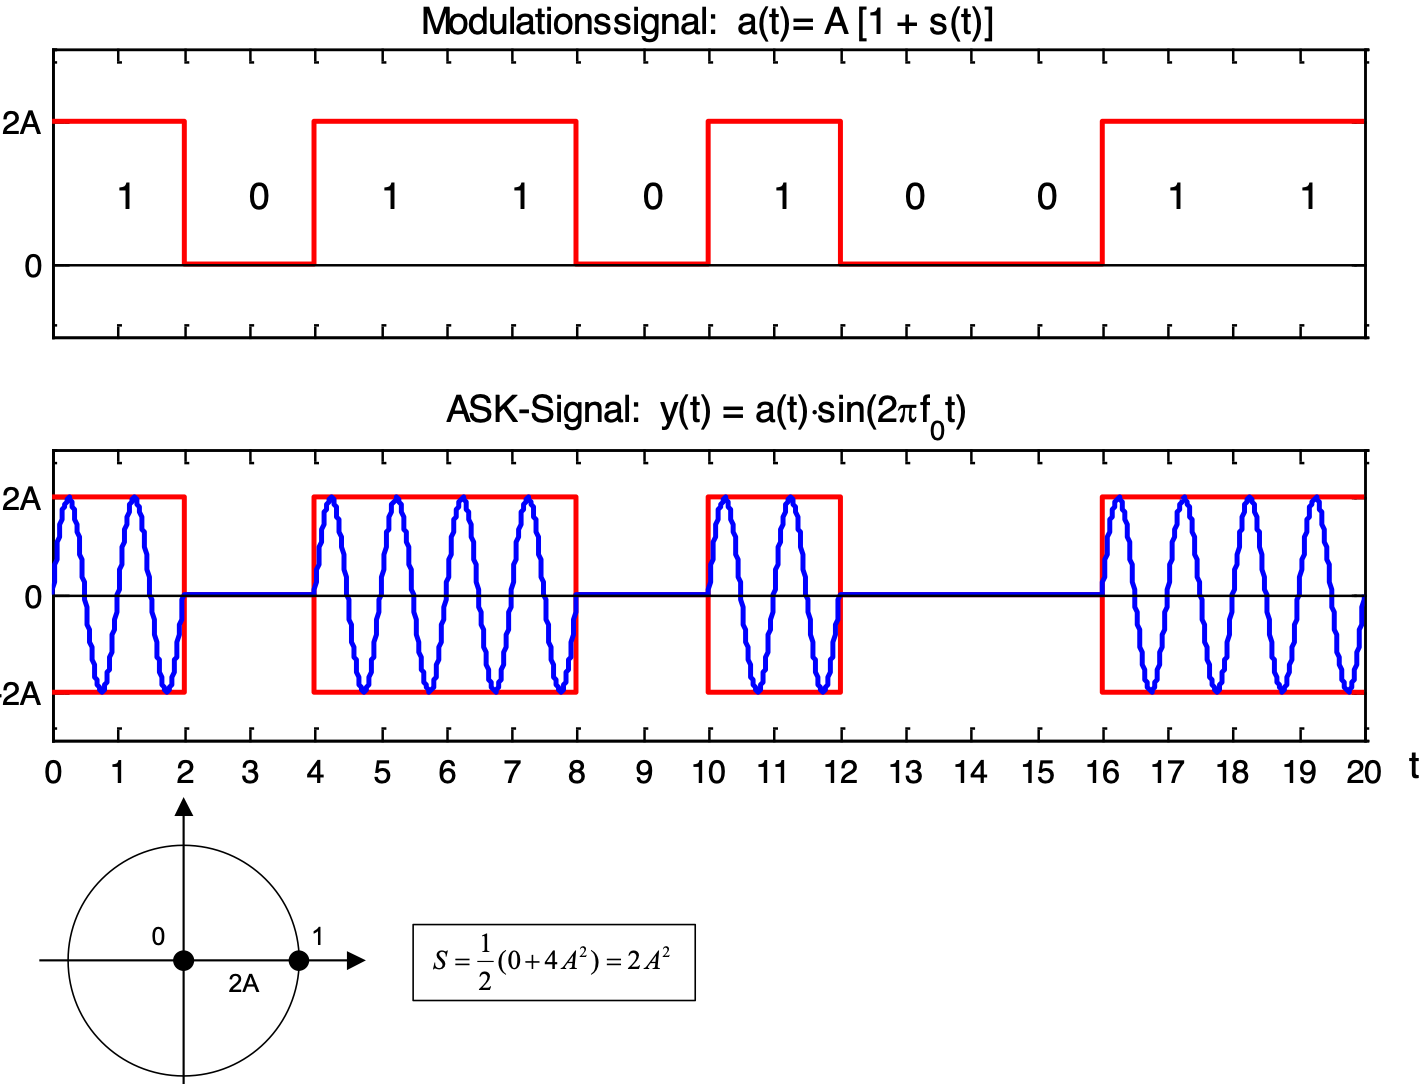
\includegraphics[width=\linewidth]{graphic/fourier/Amplitudenumtastung.png}
\end{center}
\vspace{-8pt}

\subsubsection{Phasenumtastung (PSK)}
\begin{center}
    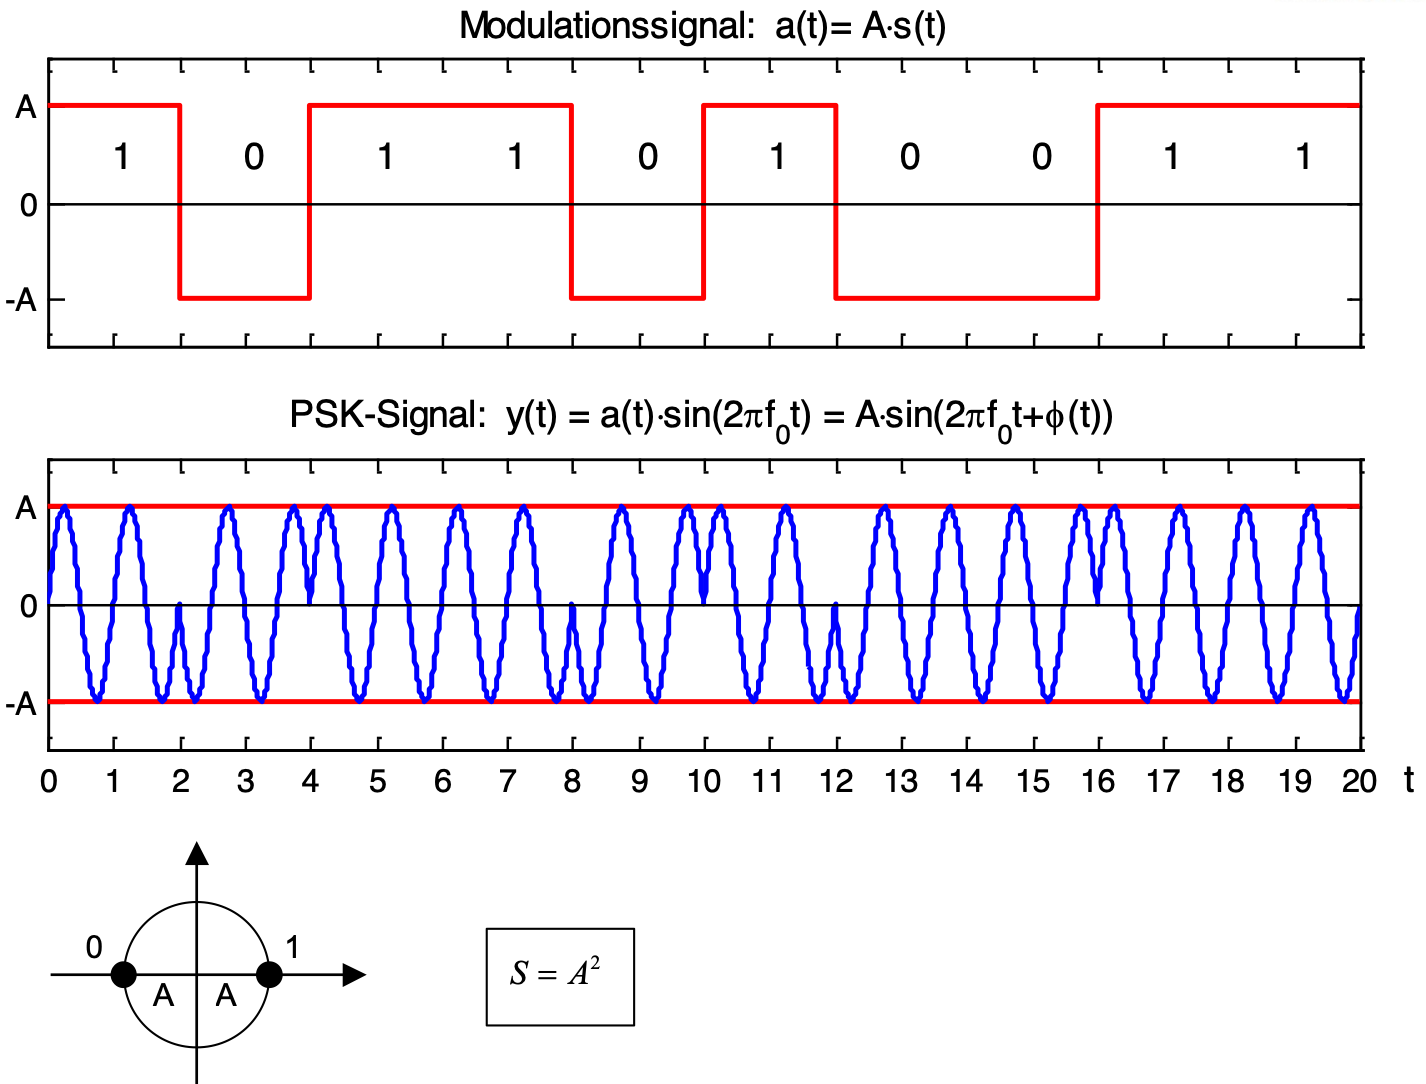
\includegraphics[width=\linewidth]{graphic/fourier/Phasenumtastung.png}
\end{center}
\vspace{-8pt}

\subsubsection{Differentielle Phasenumtastung (DPSK)}
\begin{center}
    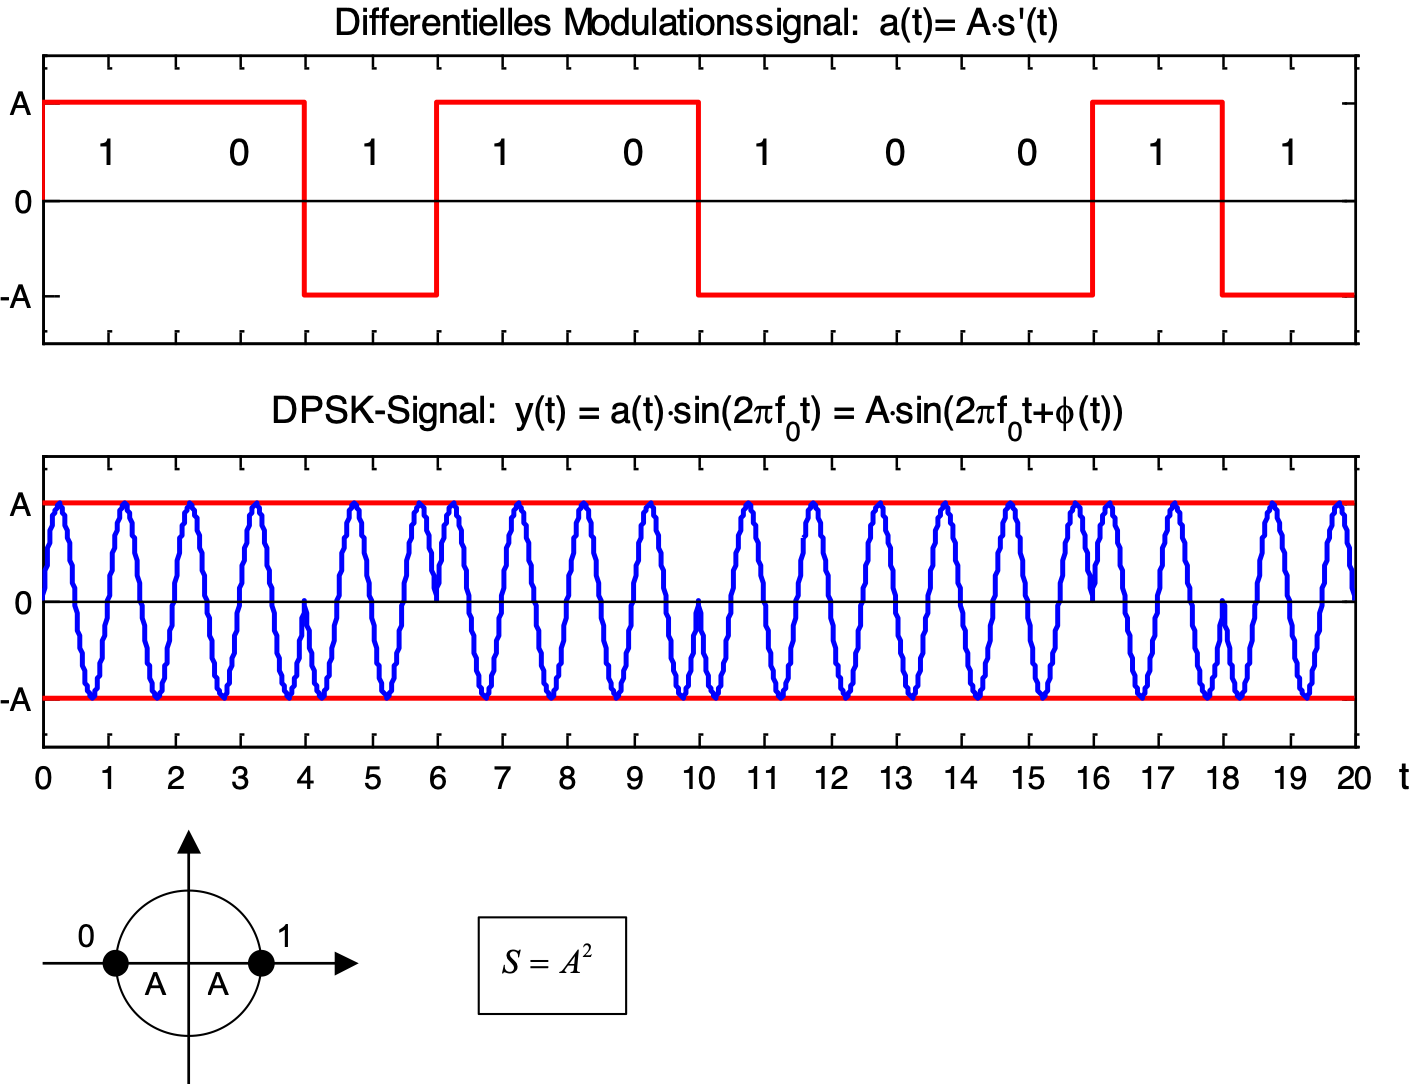
\includegraphics[width=\linewidth]{graphic/fourier/Differentielle Phasenumtastung.png}
\end{center}
\vspace{-8pt}

\subsubsection{Mehrstufige Amplitudenumtastung (PAM)}
\begin{center}
    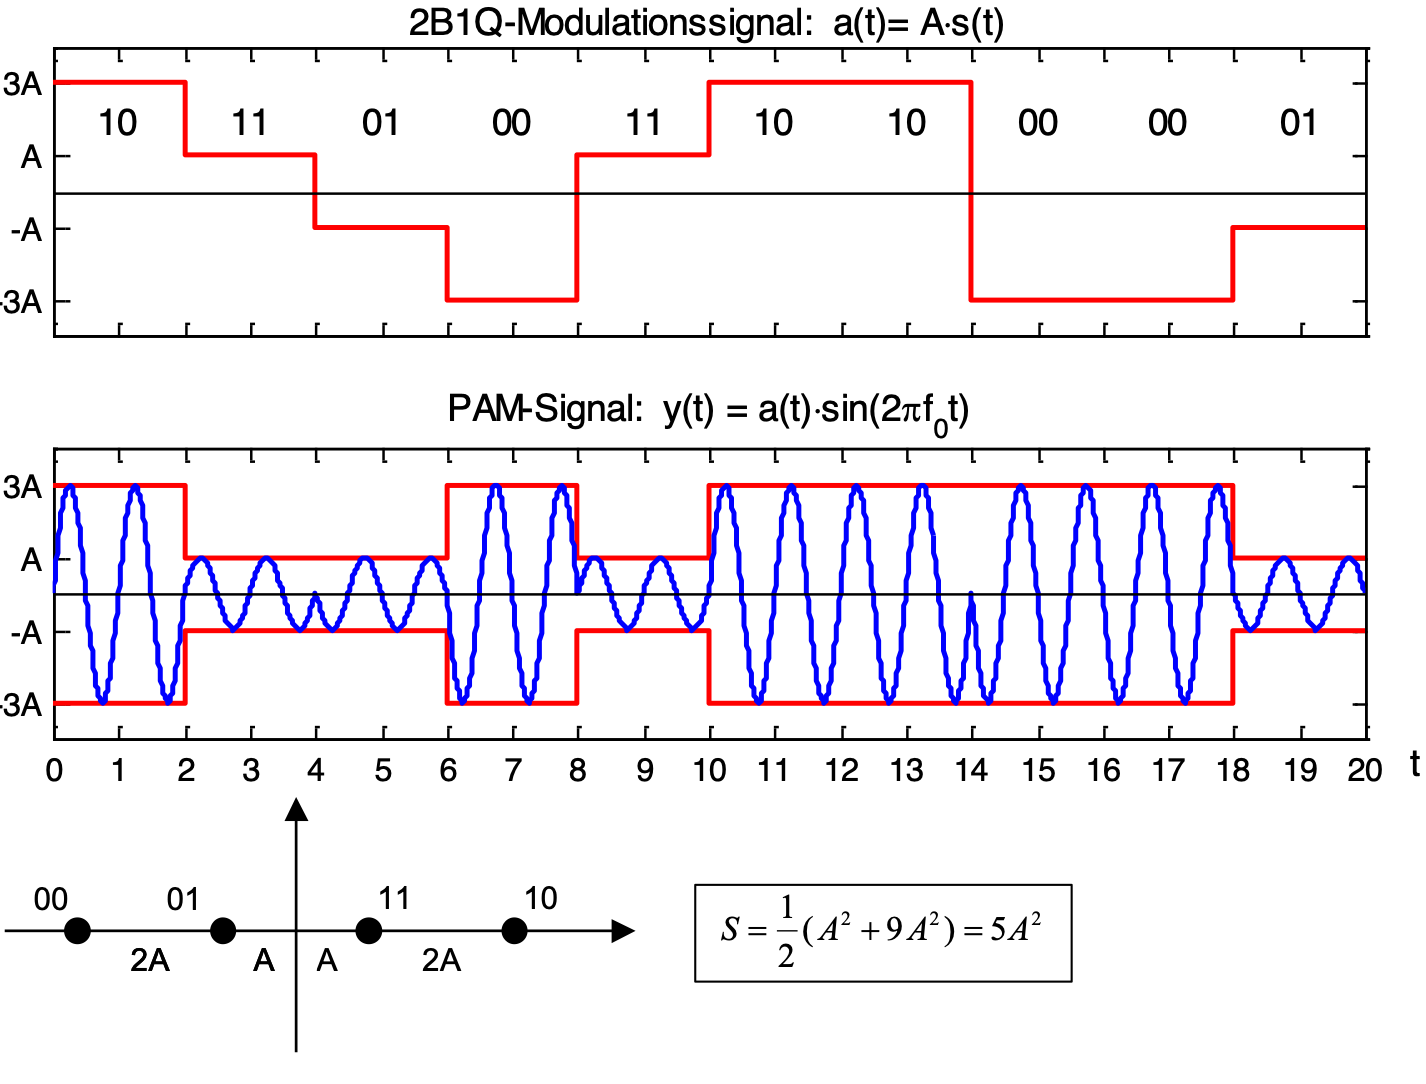
\includegraphics[width=\linewidth]{graphic/fourier/Mehrstufige Amplitudenumtastung.png}
\end{center}
\vspace{-8pt}

\subsubsection{Mehrstufige Phasenumtastung (QPSK)}
\begin{center}
    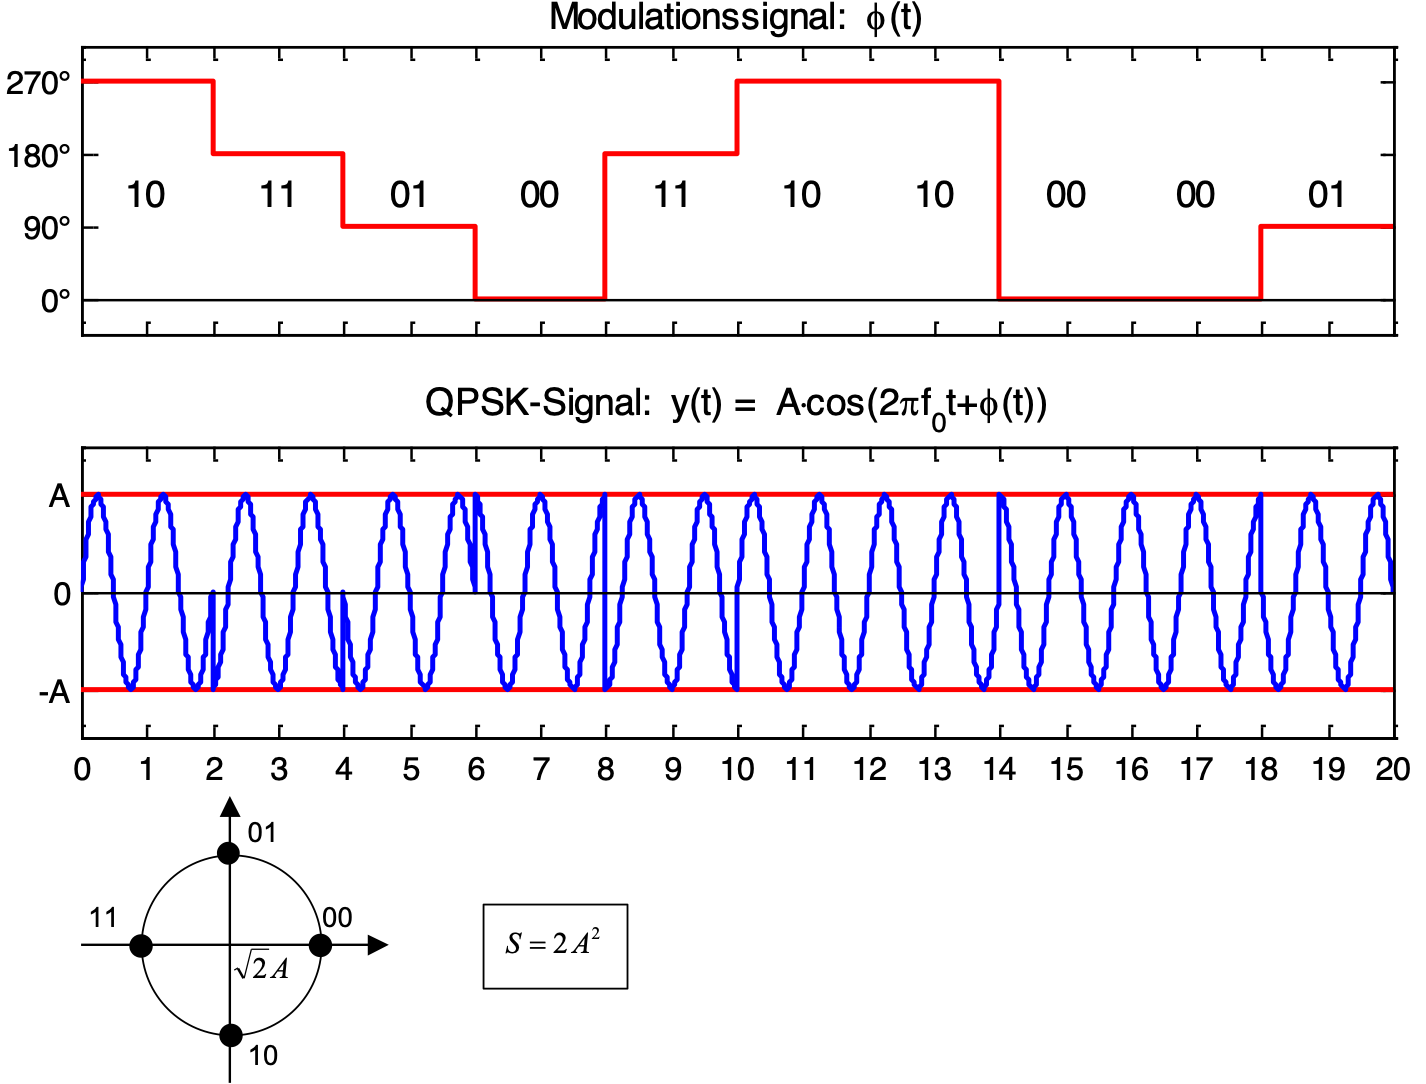
\includegraphics[width=\linewidth]{graphic/fourier/Mehrstufige Phasenumtastung.png}
\end{center}
\vspace{-8pt}


\subsubsection{QAM}
\begin{center}
    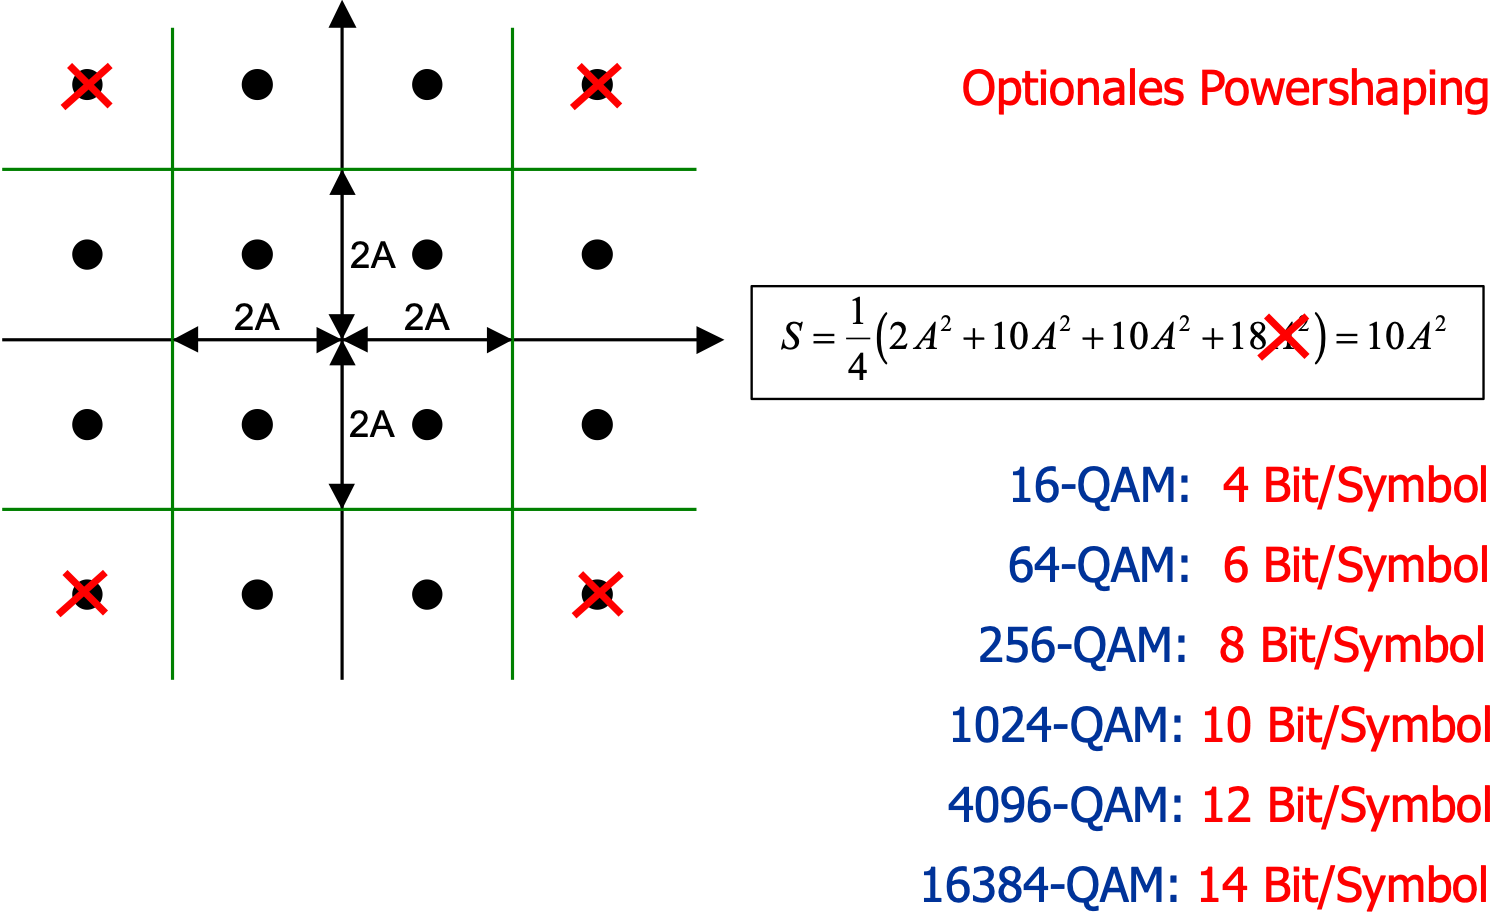
\includegraphics[width=\linewidth]{graphic/fourier/QAM.png}
\end{center}
\vspace{-8pt}

	%! Author = mariuszindel
%! Date = 25.01.21

\section{Abtasten}

\subsection{Abtasttheorem}
Damit keine Spektrumsüberlappungen (engl. Aliasing) beim Abtasten auftreten, muss die zweiseitige Bandbreite B des abzutastenden Signals kleiner als die Abtastfrequenz $f_s$
sein.\\
Dies bedeutet, dass die grösste im Spektrum vorkommende Frequenz kleiner als die Hälfte der Abtastfrequenz sein muss.\\
$B<f_s$ oder $f_{max} < f_s / 2$

\subsection{Abgetasteter zeitdiskreter Reckteckpuls}
\begin{center}
    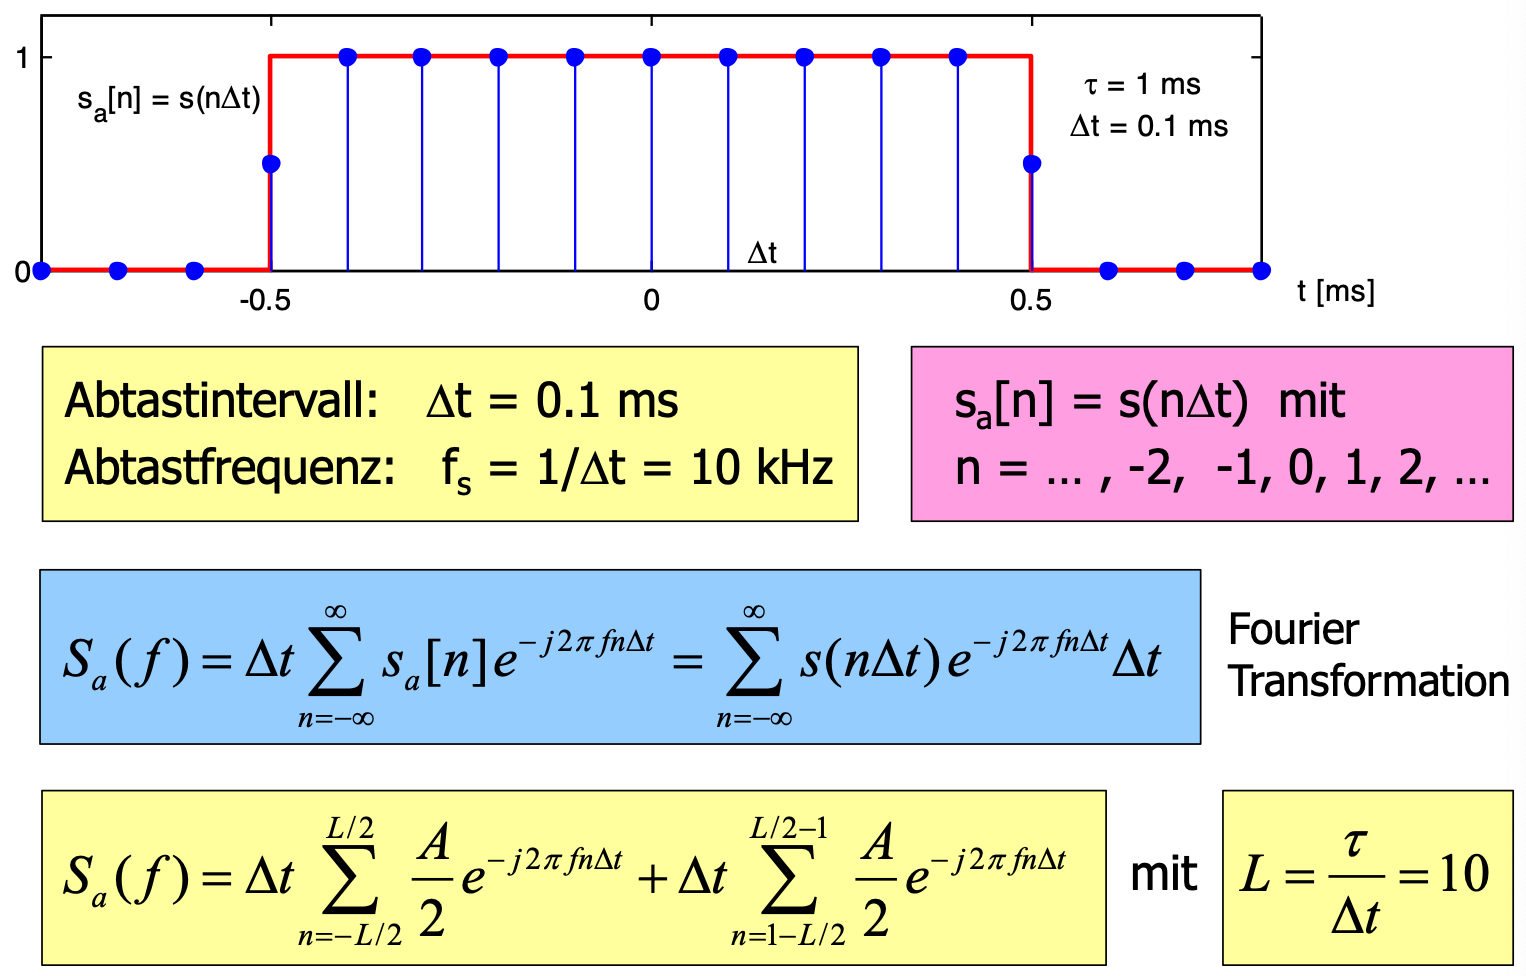
\includegraphics[width=\linewidth]{graphic/sprache-digitalisieren/Abgetasteter zeitdiskreter Reckteckpuls.png}
\end{center}
\vspace{-8pt}
Was bewirkt die gezielte Wahl der Smapling Frequenz $f_s = f_0$? Antwort: Das Sampling mit der Trägerfrequenz $f_0$ bewirkt eine Verschiebung des Datensignals in das Basisband und damit eine Produktdemodulation mit $f_0$.


\subsection{Aliasing}
Damit Frequenzkomponenten, die Aliasing verursachen, genügend unterdrückt werden können, muss die Grenzfrequenz $f_g$des Tiefpassfilters ca. 10\% unter derhalben Abtastfrequenz $f_s/ 2$ liegen.
$\rightarrow$ Aliasing tritt auf, wenn im abzutastenden Signal Frequenzanteile vorkommen, die höher sind als die halbe Abtastfrequenz. $Signal > 1/2 \times Abtastfrequenz$. Durch vorschalten eines Tiefpassfilters mit einer Grenzfrequenz $f_g < f_s / 2$, kann Aliasing vermieden werden.
\vspace{-8pt}
\begin{center}
    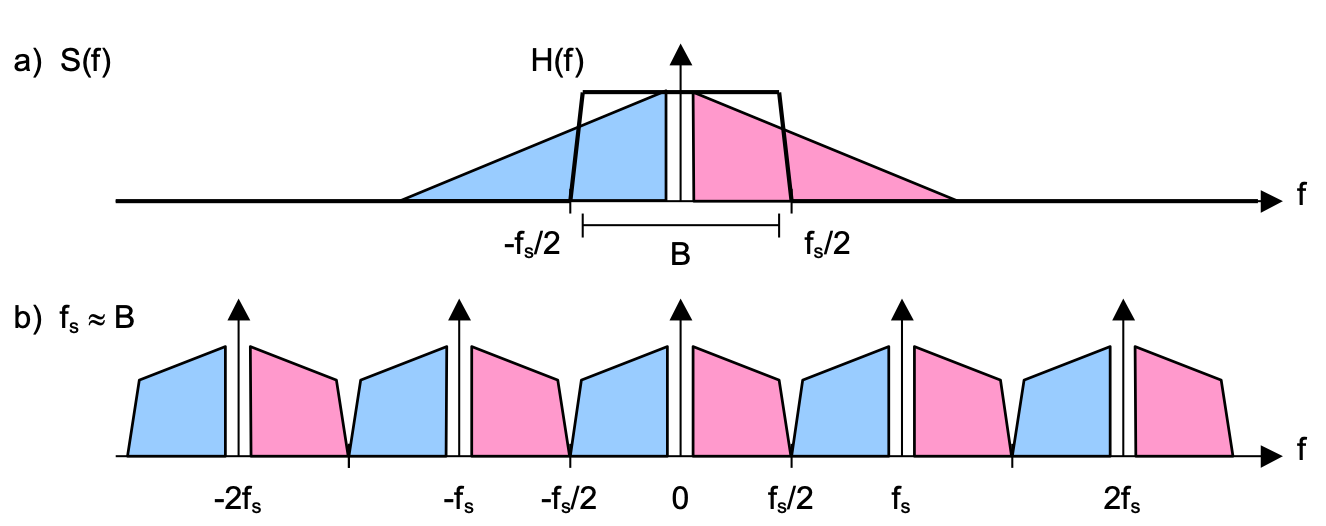
\includegraphics[width=\linewidth]{graphic/sprache-digitalisieren/Aliasing.png}
\end{center}
\vspace{-8pt}


	%! Author = mariuszindel
%! Date = 25.01.21

\section{Modulationsverfahren}
	%! Author = mariuszindel
%! Date = 25.01.21

\section{Wahrscheinlichkeit}

\subsection{Wahrscheinlichkeitsrechnung}
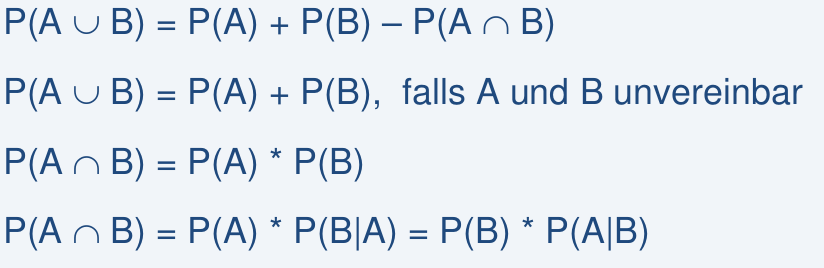
\includegraphics[width=\linewidth]{graphic/extern-reto/Wahrscheinlichkeit.png}
Lotto:\\
\colorbox{lightlightgrey}{$\frac{\binom{Gezogene}{Treffer} * \binom{Nicht-Gezogene}{Falsche}}{Anzahl aller Ergebnisse}$}\\



\subsection{Bitfehler}
\colorbox{lightlightgrey}{$P(Fehlerhaft) = 1 - P(0 Fehler)$}\\
$= 1 - $P(BitFehler)$^{Datenblock}$



\subsection{Binominalverteilung}
Wie gross ist die Wahrscheinlichkeit, dass:
\begin{itemize}
    \item genau 3
    \item weniger als 3
\end{itemize}
\colorbox{lightlightgrey}{$P(X = k) = \binom{n}{k} p^k(1 - p)^{n-k}$}\\
Wenn z.B. $\le$ 3 gesucht ist, muss für (k = 0) + (k = 1) + (k = 2) + (k = 3) gerechnet werden.


	%! Author = mariuszindel
%! Date = 25.01.21

\section{Grundlagen}




\subsection{Entscheidungsfluss}
Der Entscheidungsfluss ist definiert als\\
\colorbox{lightlightgrey}{$H_{0}^{*}=\frac{\log _{2}(N)}{\tau}\left[\frac{b i t}{s}\right]$} \\
wobei $\tau$ die Zeit ist, die zur Übertragung eines Quellzeichens benötigt wird.


\subsection{Informationsgehalt $I(x_k)$}
Der Informationsgehalt eines Zeichens sagt aus, wie viele Elementarentscheidungen zur Bestimmung dieses Zeichens zu treffen sind.
\colorbox{lightlightgrey}{$\textcolor{blue}{I(x_k)} = -log_2(P(x_k))$}


\subsection{Entropie H(X)}
Der Informationsgehalt eines Zeichens sagt aus, wie viele Die Entropie bezeichnet den mittleren Informationsgehalt der Quelle. Sie Elementarentscheidungen zur Bestimmung dieses Zeichens zu treffen zeigt also auf, wie viele Elementarentscheidungen die Quelle/Senke im Mittel sind.\\
\colorbox{lightlightgrey}{$\textcolor{blue}{H(X)} = \sum_{k = 1}^{N}p(x_k) * I(x_k)$} [bit/Zeichen]\\
Die Entropie wird maximal, wenn jedes Zeichen gleichwahrscheinlich ist!





















\subsection{Codierungstheorem von Shannon}
\colorbox{lightlightgrey}{$H(x)<L<H(x) + 1$}

\subsection{Quellen ohne Gedächnis}
Allgemein kann nicht von einer gedächtnislosen Quelle ausgegangen werden!




\subsection{Quellen mit Gedächnis (Markov-Quelle)}
\subsection{Bedingte Wahrscheinlichkeit $P(Y|X)$}
\begin{center}
\begin{tabular}{ |c|c|c|c| }
    \hline
    P(Y$|$X) & y1 & y2 & y3\\
    \hline
    x1 & $(x_1,y_1)$ & $(x_1,y_2)$ & $(x_1,y_3)$\\
    \hline
    x2 & $(x_2,y_1)$ & $(x_2,y_2)$ & $(x_2,y_3)$\\
    \hline
    x3 & $(x_3,y_1)$ & $(x_3,y_2)$ & $(x_3,y_3)$ \\
    \hline
\end{tabular}
\end{center}

\colorbox{lightlightgrey}{P(x1) = $P(x1) \times (x_1,y_1) + P(x2) \times (x_2,y_1) $}\\\colorbox{lightlightgrey}{$ + P(x3) \times (x_3,y_1)$}\\\\
\colorbox{lightlightgrey}{P(x2) = $P(x1) \times (x_1,y_2) + P(x2) \times (x_2,y_2) $}\\\colorbox{lightlightgrey}{$ + P(x3) \times (x_2,y_3)$}\\\\
\colorbox{lightlightgrey}{P(x3) = $P(x1) \times (x_1,y_3) + P(x2) \times (x_3,y_2) $}\\\colorbox{lightlightgrey}{$ + P(x3) \times (x_3,y_3)$}\\\\
\colorbox{lightlightgrey}{1 = P(x1) + P(x2)+ P(x3)}\\
Das ganze ist ein Gleichungssystem und muss nach P(x1), P(x2) und P(x3) aufgelöst werden!


\subsection{Verbundwahrscheinlichkeit $P(X,Y)$}
\begin{center}
\begin{tabular}{ |c|c|c|c| }
    \hline
    P(X$,$Y) & y1 & y2 & y3\\
    \hline
    x1 & $(x_1,y_1)$ & $(x_1,y_2)$ & $(x_1,y_3)$\\
    \hline
    x2 & $(x_2,y_1)$ & $(x_2,y_2)$ & $(x_2,y_3)$\\
    \hline
    x3 & $(x_3,y_1)$ & $(x_3,y_2)$ & $(x_3,y_3)$ \\
    \hline
\end{tabular}
\end{center}\\

\colorbox{lightlightgrey}{$P(X,Y) = P(X_i) * P(Y_k | X_i)$}\\
$P(Y_k | X_i) = $ Zellen aus Tabelle der bedingten Wahrscheinlichkeit


\subsubsection{Verbundentropie $H(X,Y)$}
Wird so berechnet, dass für jede Zeile in der Tabelle von P(X,Y), die Entropie(\colorbox{lightlightgrey}{$P(x_i,y_i)*-log_2(P(x_i, y_i))$}) berechnet und am schluss alles Addiert wird(Beachte obwohl addiert wird hat es immer ein $-$MINUS! dazwischen!).\\
\colorbox{lightlightgrey}{$-P(x1,y1) * log_2(P(x1,y1)) - P(x2,y2) * log_2(P(x2,y2)$ usw.}
\subsubsection{Bedingte Entropie $H(Y|X)$}
\colorbox{lightlightgrey}{$H(Y|X) = H(X,Y) - H(X)$}











\vfill
$$

	%! Author = mariuszindel
%! Date = 25.01.21

\section{Kompression}


\subsection{Huffman}
Berechnung der mittleren Code Wortlänge =\\ \colorbox{lightlightgrey}{$P(x)*L(x)$} Auftrittswahrscheinlichkeit * Bitlänge des Zeichens


\subsection{Codierung}


\subsubsection{DNA}
Anzahl gleiche Buchstaben + Buchstaben $\rightarrow$ aaaxxc = 3a2xc


\subsubsection{Bit-Folgen}
Bestimmen mit welchem Wert(0 oder 1) man beginnt und dann nur die Anzahl der Folge aufschreiben\\
000111010 $\rightarrow$ Beginnen mit 0 = 3 3 1 1 1\\Da die 3 mit 2 Bits dargestellt werden kann, muss man die Zeichenfolge mit 2 Bits darstellen:(Beginnend mit dem ausgewähltem Wert als 1 Bit)\\
0 11 11 01 01 01




\vfill
$$
\columnbreak
	\input{content/11-Verschlüsselung.tex}
	%! Author = mariuszindel
%! Date = 25.01.21

\section{Kanalmodell}
	%! Author = mariuszindel
%! Date = 25.01.21

\section{Block Code}


\subsection{Hammingdistanz $h$}
\begin{itemize}
    \item sicher korrigierbarer Fehler, wenn
    \item $m$ = Nachrichtenstellen
    \item $k$ = Kontrollstellen
\end{itemize}
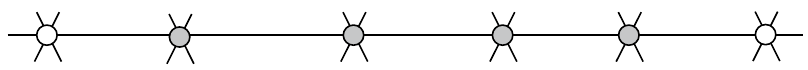
\includegraphics[width=\linewidth]{graphic/extern-reto/Hammingdistanz.png}
Jeder Knoten ist ein \textcolor{red}{Codewort}!\\
Sichere Erkennung von 4 Fehlern $\rightarrow$ Hammingdistanz = 5

\subsubsection{Anzahl aller Codeworte}
$n$ = Anzahl aller Spalten
\colorbox{lightlightgrey}{alle Codeworte = $2^n$}

\subsubsection{Anzahl gültige Codeworte}
$m$ = Anzahl Spalten der Prüfmatrix bis zur Einheitsmatrix\\
\colorbox{lightlightgrey}{gültige Codeworte = $2^m$}

\subsubsection{Sicher korrigierbarer Fehler}
$h$ \textcolor{red}{ungerade}: \colorbox{lightlightgrey}{$e = \frac{h - 1}{2}$}\hspace{3cm}\\
$h$ \textcolor{red}{gerade}: \colorbox{lightlightgrey}{$e = \frac{h - 2}{2}$}

\subsubsection{Dichtgepackt}
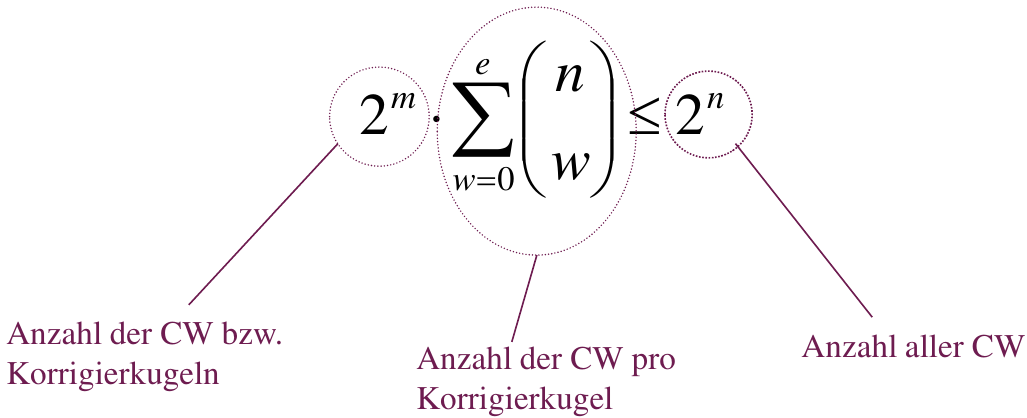
\includegraphics[width=\linewidth]{graphic/extern-reto/Dichtgepackt.png}\\
Wenn linker Teil = rechter Teil, Coderaum ist \textcolor{red}{Dichtgepackt}
\textit{Nspire: nCr(n,w)}

\subsubsection{Anzahl der Kontrollstellen $k$}
Bei Hammingcodes markiert die Einheitsmatrix in der Prüfmatrix die Anzahl der Kontrollstellen \colorbox{lightlightgrey}{$k = $ Spalten der Einheitsmatrix}

\subsubsection{Generatormatrix erstellen}
\begin{center}
    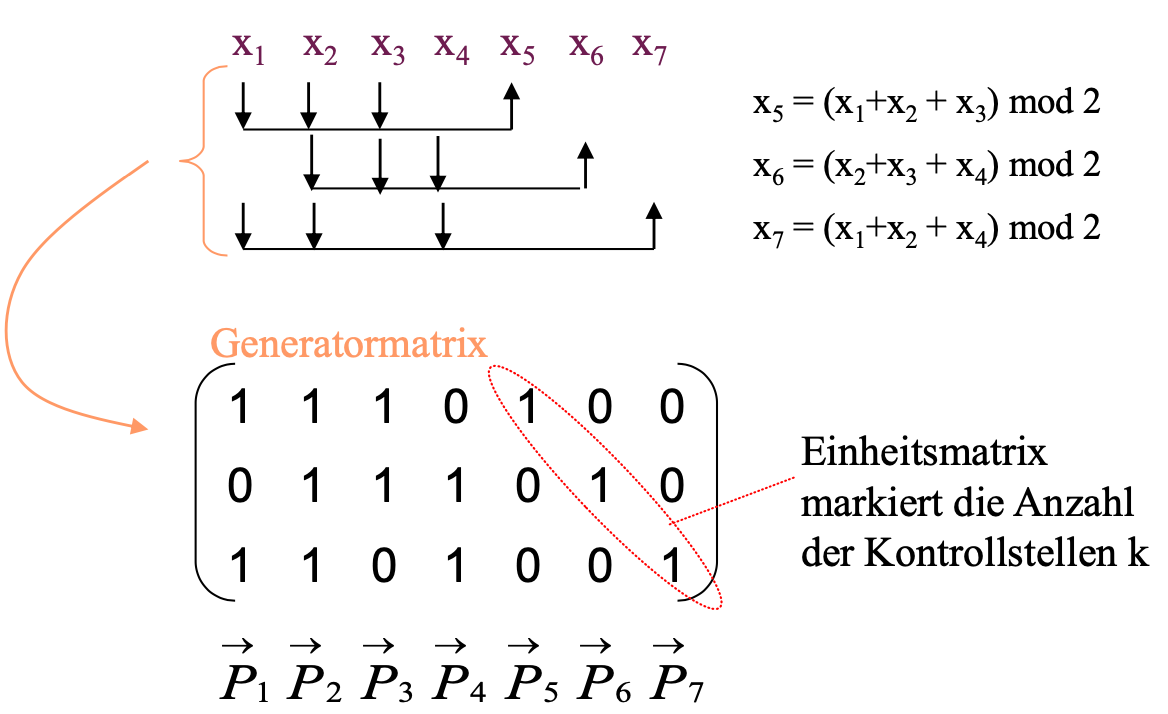
\includegraphics[width=\linewidth]{graphic/blockcode/generatormatrix.png}
\end{center}
\vspace{-8pt}



\subsubsection{Kontrollstellen ermitteln (Version 1)}
1. Grad bestimmen (xxxx), 2. Generator bestimmen(11101), 3. Wort bestimmen(100)\\
\vspace{-8pt}
\begin{center}
    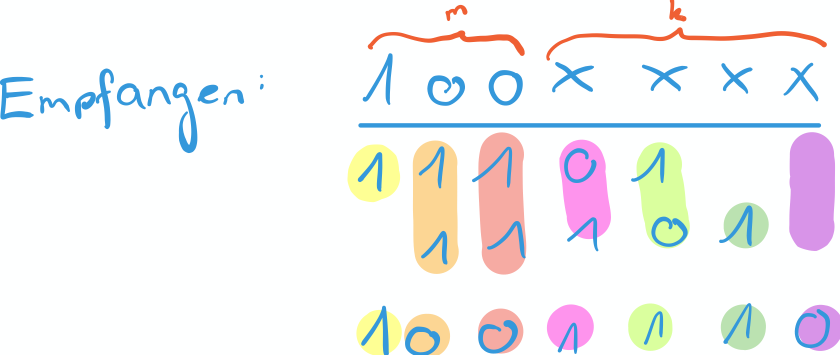
\includegraphics[scale=.3]{graphic/blockcode/kontrollstellen.png}
\end{center}
\vspace{-8pt}

\subsubsection{Kontrollstellen ermitteln (Version 2)}
1. Prüfmatrix gegeben, 2. Kontrollstellen k herauslesen (xxx), 3. Wort bestimmen(1000)\\
$(x_5 = x_1 + x_2 + x_3) mod 2$\\
$(x_6 = x_2 + x_3 + x_4) mod 2$\\
$(x_7 = x_1 + x_2 + x_4) mod 2$\\
Siehe auch Generatormatrix erstellen

\subsubsection{Fehlersyndrom bestimmen}
Bsp: $x_3$ ist gestört: Vektor $P_3$ aus Matrix lesen\\
Bsp: $x_3$ und $x_7$ ist gestört: Vektor $P_3 und P_7$ aus Matrix lesen und addieren mod 2\\




\subsection{Zyklischer Code}
Generatormatrix kann durch Generatorpolynom beschrieben werden\\
Das Codewortpolynom ist ohne Rest durch das Generatorpolynom teilbar (in mod-2-Rechnung)

\subsubsection{Grad bestimmen}
\colorbox{lightlightgrey}{$Grad = hoechste potenz$}

\subsubsection{Zyklische Abramson-Codes}
Diese werden gebildet durch die Multiplikation eines primitven Polynoms mit dem Term (1+x)
\colorbox{lightlightgrey}{$Abramson-Code: g(x)= p(x) (1+x)$}


\subsubsection{Gültige Codeworte mit Mehrfachaddition}
Grad des Generatorpolynoms entspricht Anzahl der Kontrollstellen k\\
$n = 2^k - 1$ und $n = m + k$
Generatorpolynom in Vektor umwandeln\\
%TODO


\subsubsection{gü̈ltige Codeworte mit Abramson}
$n = 2^{k-1} - 1$


\vfill
$$
\columnbreak
	%! Author = mariuszindel
%! Date = 25.01.21

\section{Faltungscodes}


\subsection{Definition}
Zur Sicherung gegen Übertragungsfehler eingesetzt.
\begin{itemize}
    \item Leichte Implementierbarkeit der Encoder und Decoder durch Schieberegister
    \item Hohe Fehlererkennungsmächtigkeit (Bündelfehlererkennung bei zyklischen Codes)
    \item Blockbildung der zu codierenden Daten notwendig
\end{itemize}


\subsection{Encoderschaltung}
Idee: Vergangenheit berücksichtigen
\vspace{-8pt}
\begin{center}
    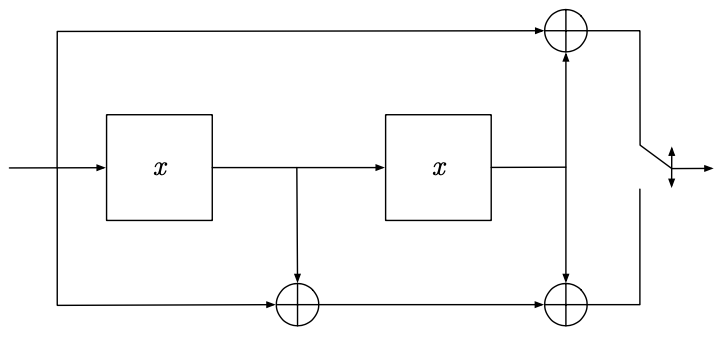
\includegraphics[scale=.33]{graphic/faltungscodes/Encoderschaltung.png}
\end{center}
\vspace{-8pt}


\subsection{Zustandsdarstellung}
\begin{center}
    \begin{tabular}{p{0.7cm} | p{0.7cm}  p{.7cm} p{.4cm} | p{.3cm} p{.1cm} | p{1cm}}
        \hline
        Eingang & Zustand & \multicolumn{2}{p{.1cm}|}{Schieberegister} & \multicolumn{2}{p{.1cm}|}{Ausgang} & Nächster Zustand \\
        \hline
        \hline
        0   &   $S_0$   &   0   &   0   &   0   &   0   &   $S_0$\\
        1   &   $S_0$   &   0   &   0   &   1   &   1   &   $S_1$\\ \hline
        0   &   $S_1$   &   1   &   0   &   0   &   1   &   $S_2$\\
        1   &   $S_1$   &   1   &   0   &   1   &   0   &   $S_3$\\ \hline
        0   &   $S_2$   &   0   &   1   &   1   &   1   &   $S_0$\\
        1   &   $S_2$   &   0   &   1   &   0   &   0   &   $S_1$\\ \hline
        0   &   $S_3$   &   1   &   1   &   1   &   0   &   $S_3$\\
        1   &   $S_3$   &   1   &   1   &   0   &   1   &   $S_3$
    \end{tabular}
\end{center}
\begin{enumerate}
    \item Tabelle mit Eingangsbits und Zuständen erstellen
    \item Ausgänge aufschreiben:
    \begin{itemize}
        \item 1. Ausgangsbit (g1) addieren Eingangsbit $+$ zweite Schieberegisterbit (mod 2)
        \item 2. Ausgangsbit (g2) addieren Eingangsbit $+$ beide Schieberegisterbit (mod 2)
    \end{itemize}
    \item Nächsten Zustand bestimmen
    \begin{itemize}
        \item Schieben der Schieberegister: Eingangsbit und erste Schieberegisterbit übernommen.
    \end{itemize}
    \item Zustandsdiagramm Zeichnen:
\end{enumerate}
\vspace{-8pt}
\begin{center}
    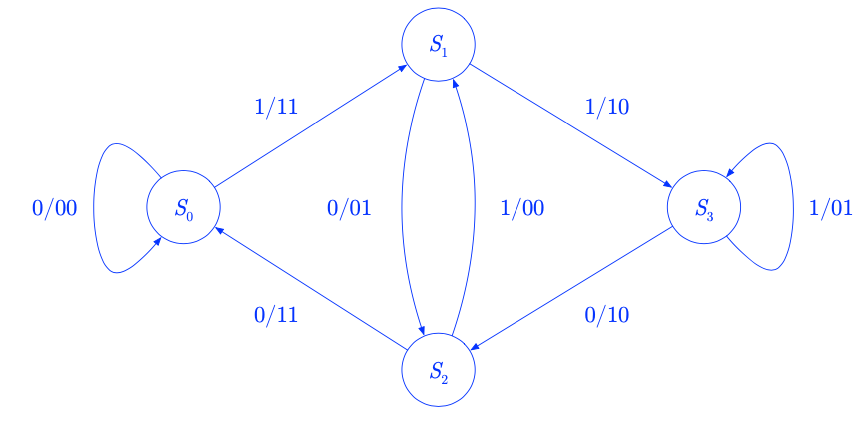
\includegraphics[scale=.3]{graphic/faltungscodes/Zustandsdiagramm.png}
\end{center}
\vspace{-8pt}

\subsection{Diverse Berechnungen}

\subsubsection{Generatorpolynome}
Hier genau zwei Polynome, da im Faltungscoder genau zwei ''Ausgänge''.\\
$g_1(x) = 1 + x^2$ (weil hinter 2. Speicher)\\
$g_2(x) = 1 + x + x^2$ (weil hinter 1. und 2. Speicher)

\subsubsection{Tailbits}
anz. Tailbits = anz. Speicherplätze

\subsubsection{Codergedächnis}

\subsubsection{Impulsantwort der Decoderschaltung}
\begin{enumerate}
    \item Beispielnachricht (${u[n]}$) einfügen (länge = anz. Speicher + 1)
    \item Durchspielen
\end{enumerate}

\subsubsection{Anzahl Zustände}
$2^n$, n=Speicherplätze

\subsubsection{Anzahl Bits für Berechnung}
Anz. = anz. Speicherplätze + aktuelle Bit

\subsubsection{Coderate bestimmen}
Anz. Ausgangsbits / Anz. Eingangsbits

\subsubsection{Block- Coderate}
$R=\frac{Eingabebits}{Anz. Ausgänge \cdot(Eingabebits + Speicherblöcke)}$

\subsubsection{Guter Code}
z.B Wenn Unterschied der Ausgabe bei Übergang immer maximal ist.



\fill
$$



\end{multicols*}

% \input{./appendix.tex}

\end{document}